\part{Tercer semestre}

\chapterimage{4.pdf} % Chapter heading image
\chapter{Ecuaciones Diferenciales}

\section{Introducción}

Dentro de las ecuaciones algebraicas, se encuentran ecuaciones en una variable,
sistemas de ecuaciones: 

\begin{itemize}
    \item Lineales
    \item No lineales
\end{itemize}

Y la solución a las ecuaciones en una variable o bien un sistema de ecuaciones son valores específicos.

\textbf{Hay tipos de ecuaciones diferenciales:}

\begin{enumerate}
    \item Ordinarias (\textbf{EDO})
    \begin{enumerate}
        \item Se considera una variables independiente
        \item una función desconocida
        \item Y sus derivadas
    \end{enumerate}
    \item En derivadas parciales
\end{enumerate}

\subsection{Ecuación diferencial Ordinaria}

\begin{definition}[Ecuación diferencial Ordinaria]
    Es una ecuación diferencial que se define como:
    \begin{equation}
        F\left(x,y,y^{\prime},y^{\prime\prime},\dots,y^{n}\right)
    \end{equation}
\end{definition}

Un ejemplo de una EDO es la siguiente:
\begin{equation*}
    y^{\prime}+y=0
\end{equation*}
donde $y=f(x)$ y $y^{\prime}=\frac{dy}{dx}$.

\subsubsection{Clasificación con respecto de la linealidad}
Considere las siguientes ecuaciones diferenciales:
\begin{example}
    $y^{\prime\prime}+y^{\prime}+2y=0$
    Es una EDO lineal.
\end{example}

\begin{example}
    $\left(y^{\prime}\right)^2+y=x$
    Es una EDO no lineal.
\end{example}

\subsubsection{Clasificación según el orden}
\begin{example}
    $y^{\prime\prime}+y^{\prime}+2y=0$
    Es una EDO lineal de segundo orden.
\end{example}

\begin{example}
    $y^{(IV)}+y=0$ 
    Es una EDO lineal del cuarto orden.
\end{example}

\subsubsection{Clasificación respecto de los coeficientes de la función desconocida y sus derivadas}
\begin{example}
    $2y^{\prime\prime}+5y^{\prime}-3y=0$
    Es una EDO lineal de segundo orden con coeficientes constantes.
\end{example}

\begin{example}
    $x^2y^{\prime\prime}+xy^{\prime}+y=0$
    Es una EDO lineal de segundo orden con coeficientes variables.
\end{example}

\subsubsection{Clasificación respecto a la homogeneidad}

\begin{example}
    $xy^{\prime\prime}+xy^{\prime}+y=\ln{(x)}$
    Es una EDO lineal de segundo orden con coeficientes variables no homogéneos.
\end{example}

\begin{definition}[No homogeneidad]
    Es una función $g(x)$ no exclusiva de la variable dependientes
\end{definition}

\subsection{Ecuación diferencial por derivadas parciales}

\begin{example}
    $\frac{\partial f}{\partial x}+\frac{\partial f}{\partial y}=0$
    Es una EDP lineal de primer orden con coeficientes constantes homogénea.
\end{example}

El primer encuentro que se ha tenido con una ecuación diferencial ordinaria, ha sido en el método de integración por partes

\begin{example}
    \begin{align*}
        &\int x\sin{(x)}\, dx&&&&\\ 
        &u=x&&dv=\sin{(x)}\, dx&&\text{Aquí se resolvió}\\
        &du=dx&&v=-\cos{(x)}+c&&\text{una ec. diferencial}
    \end{align*}
\end{example}
Al analizar la expresión $dv=\sin{(x)}\,dx$ se observa que ésta expresión es equivalente a: 
\begin{align*}
    &\frac{dv}{dx}=\sin{(x)}\implies &&v^{\prime}=\sin{(x)}\\
    &                                &&y^{\prime}=g(x)
\end{align*}

al obtener $v=-\cos{(x)}+c$ es una familia paramétrica de funciones, donde no se encuentran valores, si no familias de funciones o funciones.

\section{Solución de ecuaciones diferenciales ordinarias}

\begin{example}
Verificar que la función $y(x)=2\sqrt{x}-\sqrt{x}\ln{(x)}$ es solución de la ecuación diferencial: $4x^2y^{\prime\prime}+y=0$
\end{example}

\textit{ Sol. }

Se deriva dos veces la ``función solución''
\begin{align*}
    &y(x)=2\sqrt{x}-\sqrt{x}\ln{(x)}\\
    &y^{\prime}(x)=\frac{1}{\sqrt{x}}-\left(\frac{\ln(x)}{2\sqrt{x}}+\frac{\sqrt{x}}{x}\right)\\
    &y^{\prime}(x)=x^{-\frac{1}{2}}-\frac{1}{2}x^{-\frac{1}{2}}\ln{(x)}-x^{-\frac{1}{2}}\\
    &y^{\prime\prime}(x)=-\frac{1}{2}x^{-\frac{3}{2}}-\left[-\frac{1}{4}x^{-\frac{3}{2}}\ln{(x)}+\frac{1}{2}x{-\frac{1}{2}}\cdot\frac{1}{x}\right]+\frac{1}{2}x^{-\frac{3}{2}}\\
    &-\frac{1}{2}x^{-\frac{3}{2}}+\frac{1}{4}x^{-\frac{3}{2}}\ln{(x)}
\end{align*}

Ahora se sustituyen la segunda derivada y función de la ecuación diferencial original: 
\begin{align*}
    &4x^2\left(-\frac{1}{2}x^{-\frac{3}{2}}+\frac{1}{4}x^{-\frac{3}{2}}\ln{(x)}\right)+2x^{\frac{1}{2}}-x^{\frac{1}{2}}\ln{(x)}=0\\
    &0=0
\end{align*}

\begin{example}
    Verificar por sustitución que la función 
    $y(x)=e^x-e^{-x}$ es solución de la ecuación diferencial: $y^{\prime}=y+2e^{-x}$
\end{example}

\textit{ Sol. }
\begin{align*}
    &y^{\prime}(x)=e^x+e^{-x}\\
    &e^x+e^{-x}=y+2e^{-x}\\
    &y=e^x+2^{-x}
\end{align*}

\subsection{Un problema de valor inicial}

Un problema de valor inicial es una ecuación diferencial con una condición evaluada en cero
$y^{\prime}+y=f(x)$ con $f(x^{\prime})$ una función definida en un intervalo $I$.

El problema de valor inicial sería $y^{\prime}+y=f(x);\, y(0)=k$
Si tuviéramos $y^{\prime\prime}+y^{\prime}+y=f(x);\, y(0)=k_1, y^{\prime}(0)=k_2$

$y^{\prime\prime\prime}+y^{\prime\prime}+y^{\prime}+y=f(x);y(0)=k_1, y^{\prime}(0)=k_2, y^{\prime\prime}(0)=k_3$
Es decir, si la derivada es de orden tres, existen tres valores iniciales

\begin{example}
    Primero verificar que la solución dada satisfaga la ecuación diferencial posteriormente determine el valor de la constante
    \begin{align*}
        &y^{\prime}+y=0&& y(x)=ce^{-x}&&y(0)=2
    \end{align*}
\end{example}

\textit{ Sol. }

Se calcula la primera derivada de la función $y(x)$ 
\begin{equation*}
    y^{\prime}(x)=-ce^{-x}
\end{equation*}

Se sustituyen $y$ y $y^{\prime}$ en la ecuación diferencial
$y^{\prime}+y=0$ y se verificará que se cumpla.
\begin{align*}
    &-ce^{x}+ce^{-x}=0&&y(x)\text{es solución}
\end{align*}

Determinar el valor de la constante $c$ aplicando $y(0)=2$\footnote{$y(0)=\begin{cases}&x=0\\&y=2\end{cases}$}
\begin{align*}
    &y(x)=xe^{-x}\implies y(0)=xe^{-x}=2\\
    &\text{es llamada también solución general ó  paramétrica}
    &c\cdot 1=2\implies c=2
\end{align*}

Finalmente la solución al problema de valor inicial es: $y(x)=2e^{-x}$

\begin{example}
    Evaluar el valor en la frontera
    \begin{align*}
        &&xy^{\prime}-3y=x^3;&&y(x)=x^3\left(c+\ln{(x)}\right);&&y(1)=17
    \end{align*}
\end{example}

\textit{ Sol. }
\begin{align*}
    &y^{\prime}(x)=x^3\left(x+\ln{(x)}\right)\\ 
    &\text{Sustituyendo en la ecuación diferencial}\\ 
    &x\left(x^3\left(c+\ln{(x)}\right)+x^2\right)-3\left(x^3\left(x+\ln{(x)}\right)\right)=\\ 
    &3x^3c+3x^3\ln{(x)}+x^3-3x^3c-3x^3ln{(x)}=x^3\\
    &\text{Se concluye que y(x) es solución}\\ 
    &y(1)=17=(1)^3\left(c+\ln{(1)}\right)\implies 17=1\left(c+0\right)\\ 
    &c=17-1\left(c+0\right)=17-1\left(0\right)=17-1=16
    &\therefore c=17
\end{align*}

\begin{example}
    \begin{align*}
        &y^{\prime\prime}+2y^{\prime}+y=0&& y(x)=c_1e^{-x}+c_2xe^{-x}&&y(0)=5&&y^{\prime}(0)=-3
    \end{align*}
\end{example}

\textit{ Sol. }

\subsection{Ecuaciones diferenciales de variables separables}

Se supondrá que se tiene una ecuación diferencial de la forma
\begin{equation}
\frac{dy}{dx}=f(x,y)
\label{eq:diferenciales}
\end{equation}
El problema es el siguiente: Dada la función $f(x,y)$ se debe encontrar todas las funciones $y(x)$ que satisfacen (\eqref{eq:diferenciales})

Entonces la ecuación diferencial de primer orden es posible resolver 

\begin{equation}
    \frac{dy}{dx}=g(x)\, \forall x\in I\mid y(x)=\int g(x)\, dx+C 
\end{equation}

Donde $C$ es una constante arbitraria

Por otro lado, si la ecuación diferencial (\eqref{eq:diferenciales}) puede escribirse como: 
\begin{equation*}
    y^{\prime}+a(x)y=0
\end{equation*}

Esa última ecuación también se puede ver como: 
\begin{equation}
    \frac{dy}{dx}=-a(x)y\,\text{ si } y\neq 0\forall x\in I
\end{equation}
Implica que:
\begin{equation*}
    \frac{\frac{dy}{dx}}{y}=-a(x);
\end{equation*}
Del lado izquierdo de la igualdad se observa que: 
\begin{align*}
    &\frac{f\left(\ln{(y)}\right)}{dx}=\frac{\frac{dy}{dx}}{y}\\
    &\frac{d\left(\ln{(y)}\right)}{dx}=-a(x)\\
    &\int \frac{d\left(\ln{\left\lvert y\right\rvert }\right)}{dx}\, dx=\int -a(x)\,dx +c_1\\
    &\ln{\left\lvert y\right\rvert }=-\int a(x)\,dx +c_1\\
    &e^{\ln{\left\lvert y\right\rvert }}=e^{-\int a(x)\,dx +c_1}\implies y(x)=e^{-\int a(x)\,dx}\cdot e^{c_1}\\
    &c_1\text{ Es constante}\implies e^{c_1}=constante=c\\
    &\therefore \left\lvert y(x)\right\rvert=ce^{-\int a(x)\,dx}\\
    &c=\left\lvert y(x)\right\rvert e^{-\int a(x)\,dx}\implies c=\left\lvert y(x)\cdot e^{-\int a(x)\,dx}\right\rvert
\end{align*}

A la expresión $y(x)=ce^{-\int a(x)\,dx}$ se le conoce como solución general de la ecuación diferencial $y^{\prime}+a(x)y=0$

\begin{example}
    Resolver la ecuación diferencial
    \begin{equation*}
        y^{\prime}+2xy=0
    \end{equation*}
\end{example}

\textit{ Sol. }
\begin{align*}
    &\frac{\frac{dy}{dx}}{y}=-2x\implies \frac{d\left(\ln{(y)}\right)}{dx}=-2x\\
    &\int \frac{d\left(\ln{(x)}\right)}{dx}\, dx=\int 2x\,dx +c\implies \ln{\left\lvert y\right\rvert}=-x^2+c\\
    &y(x)=ce^{-\left(x\right)^2}\text{Solución general de }y^{\prime}+2xy=0\\
\end{align*}
Comprobación, se deriva la solución:
\begin{align*}
    &y^{\prime}(x)=-2xc\cdot e^{\left(-x^{2}\right)}\\
    &\therefore y(x)=ce^{-\left(x\right)^2}\text{ Si es solución}
\end{align*}

\subsection{Ecuaciones diferenciales de variables separables}

Una ecuación diferencial de variables separables tiene la forma:

\begin{equation}
    f_1(x)\phi_1(y)\, dx+f_2(x)\phi_2(y)\, dy=0
\end{equation}

Es posible resolverla mediante el procedimiento mediante el procedimiento de separación de variables
\begin{equation*}
    f_1(x)\phi_1(y)\, dx=-f_2(x)\phi-2(y)\, dy
\end{equation*}

Siempre y cuando $f_2(x\neq 0\, \forall x\in I)$
\begin{equation*}
    \frac{f_1(x)}{f_2(x)}\phi_1(y)\,dx=-\phi_2(y)\, dy
\end{equation*}

Siempre y cuando $\phi_2(y)\neq 0\, \forall y\in imagen\, y=f(x)\, \forall c\int I$, integrando ambos lados de la ecuación: 
\begin{equation*}
\int\frac{f_1(x)}{f_2(x)}\, dx+\int \frac{\phi_2(y)}{phi_1(y)}\,dy=C;\, Constante
\end{equation*}

\begin{example}
    Hallar la solución de la ecuación diferencial:
    \begin{equation*}
        y^{\prime}\cos{(x)}-\frac{y}{\ln{(y)}}=0
    \end{equation*}
\end{example}

\textit{ Sol. }

Se reconoce que $y^{\prime}=\frac{dy}{dx}$ entonces:
\begin{align*}
    &\frac{dy}{dx}\cos{(x)}=\frac{y}{\ln{(y)}}\\
    &\ln{(y)}\, dy=\frac{y}{\cos{(x)}}\, dx\\
    &\frac{\ln{(y)}}{y}\, dy=\frac{1}{\cos{(x)}}\implies -\frac{1}{\cos{(x)}}\, dx=\frac{\ln{(y)}}{y}\, dy=0
\end{align*}

Integrando ambos lados de la ecuación:
\begin{align*}
    &-\int\frac{dx}{\cos{(x)}}+\int\frac{\ln{(y)}}{y}\, dy=C\\
    &u=\ln{(y)}\implies du=\frac{dy}{y}\\
    &-\int \sec{(x)}\,dx+\int u\, du=C\\
    &-\ln{\left\lvert \sec{(x)}+\tan{(x)}\right\rvert}+\frac{1}{2}u^2=C\\
    &-\ln{\left\lvert \sec{(x)}+\tan{(x)}\right\rvert}+\frac{1}{2}\ln^2{(y)}=k
\end{align*}

\begin{example}
    Resolver el problema de valor inicial
    \begin{equation*}
        \left(1+e^{2x}\right)y^2\,dy=e^x\,dx\quad y(0)=0
    \end{equation*}
\end{example}

\textit{ Sol. }
\begin{align*}
    &-\frac{e^2}{1+(e^2)^2}\, dx+y^2\, dy\implies -\int \frac{e^x}{1+\left(e^x\right)^2}+\int y^2\, dy=C\\
    &u=ex\implies du=e^x\, dx\\
    &\int \frac{du}{1+u^2}+\int y2\, dy=C=-1\arctan{\left(\frac{u}{1}\right)}+\frac{1}{3}y^3=C\\
    &*\arctan{(e^x)}+\frac{1}{3}y^3=c
\end{align*}
Aplicando la condición inicial:
\begin{align*}
    &y(0)=0\implies x=0\land y=0\\
    &-\arctan(e^0)+\frac{1}{3}\cdot 0^3=c\implies -\arctan{(1)}=C\\
    &\therefore C=-\frac{\pi}{4}
\end{align*}

Por lo tanto la solución al p.v.i. será: 
\begin{equation*}
    -\arctan{(e^x)}+\frac{1}{3}\cdot y^3=-\frac{\pi}{4}
\end{equation*}

\begin{example}
    Resolver la ecuación diferencial
    \begin{equation*}
        y^{\prime}+\sin{(x+y)}=\sin{(x-y)}
    \end{equation*}
\end{example}

\textit{ Sol. }
Ésta ecuación diferencial es equivalente a:
\begin{align*}
    &\frac{dy}{dx}+\sin{(x)}\cos{(y)}+\cos{(x)}\sin{(y)}=\sin{(x)}cos{(y)}-\cos{(x)}\sin{(x)}\\
    &\frac{dy}{dx}=-2\cos{(x)}\sin{(y)}\implies \frac{dy}{\sin{(x)}}=-2\cos{(x)}\\
    &2\int \cos{(x)}\, dx+\int \csc{(y)}\, dy=C\\
    &=2\sin{(x)}+\ln{\left\lvert \csc{(y)}-c\tan{(y)}\right\rvert}=C
\end{align*}

\subsection{Ecuación diferencial a(x)y'+b(x)y=c(x)}

Para resolver la ecuación diferencial $a(x)y^{\prime}+b(x)y=c(x)$ es necesario que $a(x)\neq 0\, \forall x\in I$ luego:
\begin{equation*}
    y^{\prime}+\frac{b(x)}{a(x)}y=\frac{c(x)}{a(x)}
\end{equation*}
Suponiendo que $p(x)=\frac{b(x)}{a(x)}$ y que $Q(x)=\frac{C(x)}{a(x)}$
entonces la ecuación diferencial (equivalente a la primera mostrada) se verá como: 
\begin{equation}
    y^{\prime}+p(x)y=Q(x)
\end{equation}
Ahora se resuelve la ecuación diferencial homogénea asociada con ésta última ecuación: 
\begin{equation*}
    y^{\prime}+P(x)y=0
\end{equation*}
Es decir, hay que resolver
\begin{equation*}
    \frac{dy}{dx}+P(x)y=0
\end{equation*}
\begin{align*}
    &\frac{dy}{dx}=-P(x)y\implies -P(x)\, dx\\
    &-P(x)\, dx+\frac{dy}{y}=0\\
    &\ln{(y)}=\int -P(x)\, dx+C_1 \implies y(x)=Ce^{\int -P(x)\, dx+C}
\end{align*}
La última expresión es solución de la ecuación de $y^{\prime}+P(x)y=0$

Ahora se supondrá que $c=c(x)$ luego la expresión cambiará a:

\begin{equation}
    y(x)=c(x)\cdot e^{-\int P(x)\, dx}
    \label{eq:ecuacion_diferencial_a_y_x}
\end{equation}

Así mismo, la ecuación \eqref{eq:ecuacion_diferencial_a_y_x}
deberá satisfacer $y^{\prime}+p(x)y=Q(x)$ para ello es necesario calcular la primera derivada.
\begin{equation*}
    y^{\prime}(x)=C^{\prime}(x)e^{-\int P(x)\,dx}-C(x)P(x)e^{-\int P(x)\,dx}
\end{equation*}
Sustituyendo en $y^{\prime}+p(x)y=Q(x)$:
\begin{align*}
    &C^{\prime}(x)e^{-\int P(x)\,dx}-C(x)P(x)e^{-\int P(x)\,dx}+P(x)c(x)e^{-\int P(x)\,dx}=Q(x)\\
    &C^{\prime}(x)e^{-\int P(x)\,dx}=Q{(x)}\implies C^{\prime}(x)=Q(x)e^{\int P(x)\,dx}\\
    &\text{Integrando en ambos lados de la ecuación}\\
    &dC=Q(x)\cdot e^{\int P(x)\, dx}\, dx\implies\\
    &\int dc=\int Q(x)\cdot e^{\int P(x)\, dx}\, dx+K\implies\\
    &C(x)=\int Q(x)\cdot e^{\int P(x)\, dx}\, dx+K\\
    &\text{Por lo tanto la solución general será:}\\
    &y(x)=c(x)e^{-\int P(x)\, dx}\\
    &y(x)=\left[\int Q(x)\cdot e^{\int P(x)\, dx}\, dx+K\right]e^{-\int P(x)\, dx}
\end{align*}

Sólo falta comprobar que $y(x)$ es la solución de la ecuación diferencial. se requiere comprobar que
\begin{equation*}
    y(x)=\left[\int Q(x)\cdot e^{\int P(x)\, dx}\, dx+K\right]e^{-\int P(x)\, dx}
\end{equation*}
satisface la ecuación diferencial $y^{\prime}+p(x)y=Q(x)$ para ello es necesario calcular la primera derivada de $y(x)$. es decir:
\begin{equation*}
    y^{\prime}(x)=Q(x)e^{\int P(x)\, dx}\cdot e^{-\int P(x)\, dx}+\left[\int Q(x)e^{\int P(x)\, dx}\, dx+k \right]\left[-P(x)e^{-\int P(x)\, dx}\right]
\end{equation*}
Simplificando se tendrá: 
\begin{equation*}
    y^{\prime}(x)=Q(x)-P(x)e^{-\int P(x)\,dx}\cdot \int Q(x)\cdot e^{\int P(x)\, dx}\, dx-kP(x)e^{-\int P(x)\, dx}
\end{equation*}
Sustituyendo $y$ y $y^{\prime}$ en la ecuación diferencial:
\begin{equation*}
    Q(x)-P(x)e^{-\int P(x)\,dx}\cdot \int Q(x)\cdot e^{\int P(x)\, dx}\, dx-kP(x)e^{-\int P(x)\, dx}+P(x)\left[\int Q(x)e^{\int P(x)\, dx}\, dx+k \right]e^{-\int P(x)\, dx}=
\end{equation*}
Desarrollando para posteriormente simplificar
\begin{align*}
    &Q(x)-p(x)e^{-\int P(x)\,dx}\cdot \int Q(x)\cdot e^{\int P(x)\, dx}\, dx-kP(x)e^{-\int P(x)\, dx}+P(x)e^{-\int P(x)\, dx}\cdot \int Q(x)e^{\int P(x)\, dx}\, dx+kP(x)e^{-\int P(x)\, dx}=\\
    &Q(x)=Q(x)\\
    &\therefore y\text{ Si es solución de } y^{\prime}+p(x)y=Q(x)
\end{align*}

\begin{problem}[Resuelva ]
    $y^{\prime}+y=x$, $y(0)=4$
\end{problem}

\textit{ Sol. }

Siguiendo el procedimiento paso a paso se obtiene:

El coeficiente de la derivada es uno, por lo tanto se resuelve la ecuación diferencial homogénea asociada a $y^{\prime}+y=0$
\begin{align*}
    &\implies \frac{dy}{dx}=-y\implies \frac{dy}{y}=-dx\implies \ln{(y)}=-x+C_1\\
    &\implies y_h(x)=Ce^{-x}
\end{align*}

$y_h(x)=Ce^{-x}$ es solución de $y^{\prime}+y=0$, ahora se supondrá que la $c=c(x)$
por lo tanto se transformará en: 

\begin{equation}
    y(x)=c(x)e^{-x}
\label{eq:y(x)=c(x)e^{-x}}
\end{equation}

Se supondrá que la ecuación \eqref{eq:y(x)=c(x)e^{-x}} es solución de $y^{\prime}+y=0$, entonces $y^{\prime}(x)=C^{\prime}(x)e^{-x}-c(x)e^{.x}$
sustituyendo ésta última, se obtiene: 
\begin{align*}
    &c^{\prime}(x)e^{-x}-c(x)e^{-x}+c(x)^{\prime}=x\implies c^{\prime}(x)e^{-x}=x\\
    &\implies c^{\prime}(x)=xe^{-x}\implies dc=xe^x\, dx\\
    &\int dc=\int xe^x\, dx+k\implies c(x)=xe^x-\int e^x\, dx=xe^x-e^x+k
\end{align*}

Por lo tanto la solución general será:
\begin{equation*}
    y(x)=\left(xe^x-e^x+k\right)e^x\implies y(x)=x-1+ke^{-x}
\end{equation*}

Para determinar el valor de la constante $k$, se sustituyen la condición inicial

para determinar el valor de la constante $k$ se aplicará la condición inicial $y(0)=4\implies x=0;\, y=4$
\begin{align*}
    &y(0)=0-1+ke^{-0}=4\implies -1+k=4\implies k=5\\
    &\text{ Por lo tanto la solución al p.v.i. sería:}\\
    &y(x)=x-1+5e^{-x}
\end{align*}

Ahora sólo falta comprobar que es solución de $y^{\prime}+y=x$, se calcula $y^{\prime}$
\begin{align*}
    &y^{\prime}=1-5e^{-x}\\
    &\text{Sustituyendo junto con }y\\
    &1-5e^{-x}+(x-1+5e^{-x})=x
\end{align*}

\begin{example}
    Resolver la ecuación:
    \begin{equation}
        x^2y^{\prime}+x(x+2)y=e^x
        \label{eq:example1}
    \end{equation}
\end{example}

\textit{ Sol. }

Cumple con $a(x)y^{\prime}+b(x)y=c(x)$, se identifica que el coeficiente de $y^{\prime}\neq 1$
entonces la ecuación diferencial \eqref{eq:example1}, se dividirá entre $x^2$ obteniendo lo siguiente: 
\begin{equation}
    y^{\prime}+\left(1\frac{2}{x}\right)y=x^{-2}e^x
    \label{eq:example2}
\end{equation}

En la ecuación diferencial \eqref{eq:example2} se identifica que: 
\begin{align*}
    &P(x)=1+\frac{2}{x}&&Q(x)=x^{-2}e^x
\end{align*}
Aplicando directamente la fórmula para la solución de una ecuación diferencial de primer orden con coeficiente de variables no homogéneas, se tiene:
\begin{align*}
    &y(x)=\left[\int Q(x)\cdot e^{\int P(x)\, dx}\, dx+k \right]e^{-\int P(x)\, dx}\\
    &y(x)=\left[\int x^{-2}e^x\cdot e^{\int
    1+\frac{2}{x})\, dx}\, dx+k  \right]e^{-\int \left(1+\frac{2}{x}\right)\, dx}\\
    &\text{Calculando las integrales por separado:}\\
    &-\int \left(1+\frac{2}{x}\right)\, dx=-\int \, dx-2\int\frac{dx}{x}=-x-2\ln{(x)}+k\\
    &e^{-x-2\ln{(x)}}=e^{-x+\ln{(x^{-2})}}\\
    &e^{-x}\cdot e^{\ln{(x^{-2})}}=e^{-x}\cdot x^{-2}
\end{align*}

La otra parte de la solución: 
\begin{align*}
    &\int x^{-2}e^x\cdot e^xx^2\, dx=\int e^{2x}\,dx=\frac{1}{2}e^{2x}+k_2\\
    &y(x)=\left[\frac{1}{2}e^{2x}+k_2 \right]e^{-x}\cdot x^{-2}=\frac{1}{2}x^{-2}e^{x}+kx^{-2}e^{-x}
\end{align*}

Ahora se comprueba que es solución 
\begin{align*}
    x^2y^{\prime}+x(x+2)y=e^x\\
    x^2\left[a\right]
\end{align*}

%%%%%%%%%%%%%%%%%%%%%%%%%%%%%%%%%%%%%%%%%%%%%%%%%%%%%%%%

\begin{example}
    Resolver la ecuación diferencial: $x^{\prime}+\frac{x}{y}=y^4$
\end{example}

\textit{ Sol. }

En éste caso, $x=x(y)$ 
Se resuelve la ecuación diferencial homogénea asociada con la ecuación del problema:
\begin{align*}
    &x+^{\prime}+frac{x}{y}=0\\
    &frac{dx}{dy}=-\frac{x}{y}\implies \frac{dx}{x}=-\frac{dy}{y}\implies ln{(x)}=-ln{(y)}+ln{(c)}\\
    &ln{(x)}=ln{\left(\frac{c}{y}\right)}
\end{align*}
Aplicando la función exponencial a ambos lados de la ecuación: 
\begin{equation*}
e^{\ln{(x)}}=e^{\left(\frac{c}{y}\right) }\implies x=\frac{c}{y}
\end{equation*}
Ahora se supondrá que $c=c(y)$ por lo tanto se transforma en: 
\begin{equation*}
    x=\frac{c(y)}{y}
\end{equation*}

Sustituyendo $x$ y sus derivadas en la ecuación diferencial:
\begin{align*}
    &x^{\prime}=\frac{c^{\prime}(y)-c(y)\cdot 1}{y^2}\\
    &=\frac{yc^{\prime}-c(y)}{y^2}
\end{align*}
La ecuación en donde deberá sustituirse $x^{\prime}+\frac{x}{y}=y^4$
\begin{align*}
    &\frac{c^{\prime}(y)}{y}-\frac{c(y)}{y^2}+\frac{\frac{c(y)}{y}}{y}=y^4\\
    &c^{\prime}(y)=y^5\implies dc=y^5\, dy\\
    &\int \,dc=\int y^5\, dy\\
    &c(y)=\frac{1}{6}y^6+k
\end{align*}
Por lo tanto la solución de la ecuación diferencial es:
\begin{align*}
    &x(y)=\frac{1}{6}y^6+k\\
    &x(y)=\frac{\frac{1}{6}y^6+k}{y}\implies x(y)=\frac{1}{6}y^5+\frac{k}{y}
\end{align*}

\section{Ecuaciones diferenciales exactas}


\begin{definition}[Ecuación diferencial exacta]
    Una expresión diferencial de la forma $M(x,y)\, dx+N(x,y)\, dy$ es una diferencial exacta sobre una región $R$ del plano $xy$ si esta proviene del diferencial de alguna función $f(x,y)$ definida sobre $R$. Luego una ecuación diferencial lineal de primer orden de la forma $M(x,y)\, dx+N(x,y)\, dy=0$ se dice ecuación exacta sí el lado izquierdo de la igualdad es una diferencial exacta.
\end{definition}

\begin{example}
    La ecuación diferencial $1xt\, dx+\left(x^2-1\right)\,dy=0$ es una ecuación diferencial exacta
\end{example}

Se identifica que $M(x,y)=2xy$ y $N(x,y)=x^2-1$ se observa $\frac{\partial M}{\partial y}=\partial x=\frac{\partial N}{\partial x}$ 
por lo tanto la ecuación diferencial es exacta
\newpage
\begin{theorem}
    Sean $M(x,y)$ y $N(x,y)$ funciones continuas y diferenciables en cierta región $R$. Una condición necesaria y suficiente
    para que $M(x,y)\, dx+N(x,y)\,dy$ sea una diferencial exacta es:   
    \begin{equation}
        \frac{\partial M}{\partial y}=\frac{\partial N}{\partial x}
    \end{equation}
\end{theorem}

Para resolver la ecuación diferencial $M(x,y)\, dx+N(x,y)\, dy=0$
Primero se verifica que la diferencial sea exacta, una vez verificado será entonces: Existe $f(x,y)\mid \frac{\partial f}{\partial x}=M(x,y)$
entonces es posible determinar $f$ si se integra $M(x,y)$ con respecto de $x$, es decir: 
\begin{align*}
    &\int \frac{\partial f}{\partial x}\, dx=\int M(x.y)\, dx+k(y)\\
    &f(x,y)=\int M(x,y), dx+k(y)
\end{align*}
Ahora se deriva $f(x,y)$ con respecto a $y^{\prime \prime}$
\begin{align*}
    &\frac{\partial f}{\partial y}=\frac{\partial}{\partial y}\left(\int M(x,y)\, dx\right)+\frac{\partial}{\partial y}\left(k(y)\right)=N(x,y)\\
    &k^{\prime}(y)=N(x,y)-\frac{\partial }{\partial y}\left(\int M(x,y)\, dx\right)\\
    &\text{Integrando respecto }y
    &dk=N(x,y)\, dy-\int \frac{\partial}{\partial y}\left(\int M(x,y)\, dx\right)\\
    &k=\int N(x,y)\, dy-\int M(x,y)\, dy\\
    &k(y)=\int N(x,y)-\int N(x,y)\, dy\\
    &f(x,y)=\int M(x,y)\, dx+\int N(x,y)\, dy-\int M(x,y)\, dx\\
    &f(x,y)=\int N(x,y)\, dy
\end{align*}


\begin{example}
    Resuelve la ecuación diferencial $e^{2y}-y\cos{(xy)}\,dx+\left(2xe^{2y}-x\cos{(xy)}+2y\right)\, dy=0$
\end{example}

\textit{ Sol. }

Se identifican los término en la ecuación diferencial 
\begin{align*}
    &M(x,y)=e^{2y}-y\cos{(xy)}\\
    &N(x,y)=2xe^{2y}-x\cos{(xy)}+2y	
\end{align*}
Y se verifican las condiciones del teorema.
\begin{align*}
    &\frac{\partial M}{\partial y}=2e^{2y}+y\sin{(xy)}-\cos{(x,y)}\\
    &\frac{\partial N}{\partial x}=2e^{2y}-\cos{(x+y)}+yt\sin{(xy)}\\
    &\therefore \frac{\partial M}{\partial y}=\frac{\partial N}{\partial x}
\end{align*}
Se cumplen las condiciones del teorema de necesidad y suficiencia; integrando $M(x,y)$ con respecto de $x$ se obtiene:
\begin{align*}
    &\int M(x,y)\, dx=\int e^{2y}-y\cos{(xy)}\\
    &=xe^{2y}-\frac{y}{y}\sin{(xy)}+k(y)\\
    &\implies f(x,y)=xe^{2y}-\sin{(xy)}+k(y)
\end{align*}
Ahora, debe cumplirse que la derivada parcial de f con respecto a y, debe ser igual a $N(x,y)$:
\begin{align*}
    &\frac{\partial f}{\partial y}=2xe^{2y}-x\cos{(xy)}+k^{\prime}(y)=2xe^{2y}-x\cos{(xy)}+2y \\
    &\therefore k^{\prime}(y)=2y\\
    &\int 2y\, dy\implies k(y)=y^2+c
\end{align*}

Por lo tanto la solución general de la ecuación diferencial es:
\begin{align*}
    &f(x,y)=xe^{2y}-\sin{(xy)}+y^2+c_1=0\\
    &\therefore x^2e^{2y}-\sin{(xy)}+y^2=c\\
\end{align*}

\begin{example}
    \begin{equation*}
        \frac{dy}{dx}=\frac{xy^2-\cos{(x)}\sin{(x)}}{y\left(1-x^2\right)}\, y(0)=2
    \end{equation*}
\end{example}

\textit{ Sol. }

Se escribe la ecuación diferencial en la forma estándar de una ecuación diferencial exacta.
\begin{equation*}
    \left(xy^2-\cos{(x)}\sin{(x)}\right)\, dx+y\left(x^2-1\right)\, dy=0
\end{equation*}
Se identifican:
\begin{align*}
    &M(x,y)=xy^2-\cos{(x)}\sin{(x)}\\
    &N(x,y)=y\left(x^2-1\right)
\end{align*}
Ahora hay que verificar la condición de necesidad y suficiencia del teorema.
\begin{align*}
    &\frac{\partial M}{\partial y}=2xy\\
    &\frac{\partial N}{\partial x}=2xy\\
    &\frac{\partial M}{\partial y}=\frac{\partial N}{\partial x}
\end{align*}
Como se cumplen las condiciones de necesidad y suficiencia, se tiene una ecuación diferencial exacta, se procede a calcular $f(x,y)$
\begin{align*}
    &f(x,y)=\int M(x,y)\, dx\\
    &=\int xy^2-\cos{(x)}\sin{(x)}\, dx\\
    &f(x,y)=\frac{1}{2}x^2y^2-\frac{1}{4}\cos{(2x)}+k(y)
\end{align*}
Ahora se calcula $\frac{\partial f}{\partial y}$ obteniendo:
\begin{align*}
    &x^2y+k^{\prime}(y)y\left(x^2-1\right)\\
    &k^{\prime}(y)=-y\\
    &k(y)=-\frac{1}{2}y^2+c\\
    &\text{La solución general de la ec.}
    &\frac{1}{2}x^2y^2-\frac{1}{4}\cos{(2x)}-\frac{1}{2}y^2=c
\end{align*}
Ahora se aplica la condición inicial $y(0)=2$
\begin{align*}
    &\frac{1}{2}(0)^2(2)^2-\frac{1}{4}\cos{\left(2(0)\right)}-\frac{1}{2}(2)^2=c\\
    &-\frac{1}{4}-2=c\implies c=-\frac{9}{4}
\end{align*}
Finalmente la solución particular de la ecuación diferencial será:
\begin{equation*}
    \frac{1}{2}x^2y^2-\frac{1}{4}\cos{(2x)}-\frac{1}{2}y^2=-\frac{9}{4}
\end{equation*}

\subsubsection{Factor de integración o factor integrante}
Se emplea cuando la ecuación diferencial $M(x,y)\, dx+N(x,y)\, dy=0$ no es exacta, es decir,
el criterio de necesidad y suficiencia no se cumple.
En el caso cuando no se satisface el criterio, la ecuación diferencial se multiplica
por un factor $\mu (x,y)$ quedando la ecuación como sigue:

\begin{equation}
    \mu (x,y)M(x,y)\, dx+\mu(x,y)N(x,y)\, dy=0
    \label{eq:factoreqdf}
\end{equation}

Con esto se pretende que la ecuación \eqref{eq:factoreqdf} sea exacta, ahora deberá
cumplirse que:
\begin{equation*}
    \frac{\partial (\mu \cdot N)}{\partial y}=\frac{\partial (\mu\cdot N)}{\partial x}
\end{equation*}
Es decir:
\begin{align*}
    &\frac{\partial\mu}{\partial y}\cdot M(x,y)+\mu \cdot \frac{\partial M}{\partial y}= \frac{\partial \mu}{\partial x}\cdot N(x,y)+\mu \cdot \frac{\partial N}{\partial x}\\
    &\mu_y \cdot M(x,y)+\mu_y \cdot M_y=\mu_x\cdot N+\mu\cdot N_x\\
    &\mu\left(M_y-N_x\right)=\mu_x\cdot N-\mu_yM
\end{align*}
\textbf{Suponiendo que M sólo depende de x} $\mu_y M=0$, 
\begin{align*}
    &M\left(M_y-N_x\right)=\mu_x\cdot N\\
    &\frac{d\mu}{dx}=\frac{\left(M_y-N_x\right)\mu}{N}
\end{align*}
Esperando que la parte del cociente anterior sólo dependa de $x$, si es pasa, la ecuación diferencial de variables separables o lineal de coeficientes variables.
\begin{align*}
    &\frac{d\mu}{\mu}=\frac{M_y-N_x}{N}\, dx\implies \\
    &\int \frac{du}{\mu}=\int \frac{M_y-N_x}{N}\, dx+k\\
    &\mu =e^{\int \frac{M_y-N_x}{N}\, dx} \text{Factor de integración}
\end{align*}
Si en la ecuación diferencial $M(x,y)\, dx+N(x,y)\, dy=0$ se tiene que: 
\begin{enumerate}
    \item $\frac{M_y-N_x}{N}$ es una función de ``$x$'', entonces el factor de integración $e^{\int \frac{M_y-N_x}{N}\, dx}$
    \item En el otro caso $\frac{N_x-M_y}{M}$ es una función de $y$, entonces el factor de integración sería $\mu(y)=e^{\int \frac{N_x-M_y}{N}\, dy}$
\end{enumerate}
\begin{example}
    Resuelva la ecuación diferencial $xy\, dx+\left(2x^2+3y^2-20\right)\, dy=0$
\end{example}

\textit{ Sol. }

Se verifica la condición de necesidad y suficiencia para la ecuación diferencial 
$M(x,y)=xy;$ $N(x,y)=2x^2+3y^2-20$
\begin{align*}
    &\frac{\partial M}{\partial y}=x&&\frac{\partial N}{\partial x}=4x
\end{align*}

La conclusión es que $\frac{\partial M}{\partial y}\neq \frac{\partial N}{\partial x}$

Por lo tanto la ecuación diferencial no es exacta. Se procede a buscar un factor que haga que sea exacta. El cual se calculará como sigue: 
\begin{align*}
    \frac{M_y-N_x}{N}=\frac{x-4x}{2x^2+3y^2-20}=\mu(x,y)
\end{align*}
Como $d\mu$ depende de dos variables, entonces no sirve esta expresión, ahora se verificará:
\begin{align*}
    \frac{N_x-M_y}{N}=\frac{4x-x}{xy}=\frac{2x}{xy}=\frac{3}{y}=\mu(y)
\end{align*}
Por lo tanto el factor de integración tendrá la forma.
\begin{align*}
    \mu(y))e^{\int \frac{3}{y}\, dx}\implies \mu(y)=e^{3\ln{(y)}}=y^3
\end{align*}
Ahora se multiplica la ecuación diferencial por el factor de integración
\begin{align*}
    y^3\left(xy\, dx+\left(3x^2+3y^2-20\right)\, dy=0\right)\\
    xy^4\, dx+\left(2x^2y^3+2y^5-2'y^3\right)\, dy=0
\end{align*}
Se verifican nuevamente la condición de necesidad y suficiencia
\begin{equation*}
    \frac{\partial M}{\partial y}=4xy^3\, \frac{\partial N}{\partial x}=4xy^3
\end{equation*}
Esta ecuación ya es exacta y es equivalente a la primera forma, para resolverla.
\begin{align*}
    &f(x,y)=\int xy^4\, dx=\frac{1}{2}x^2y^4+k(y)\\
    &\frac{\partial f}{\partial y}=2x^2y^3+k^{\prime}(y)=2x^2y^3+3y^5-20y^3\\
    &k^{\prime}(y)=3y^5-20y^3\\
    &k(y)=\frac{1}{2}y^6-5y^4+c_1\\
    &\therefore \frac{1}{2}x^2y^4+\frac{1}{2}y^6-5y^4=c
\end{align*}

\begin{example}
    Resolver la ecuación diferencial
    \begin{equation*}
    \left( x\cos{y} -y\sin{(y)}\right)\, dy+\left( x\sin{(y)}+y\cos{(y)} \right)\, dx=0
    \end{equation*}
\end{example}

\textit{ Sol. }

Se verifica si se tiene una ecuación diferencial exacta. Se identifican:
\begin{align*}
    &M(x,y)=x\sin{(y)}+y\cos{(y)}\\
    &N(x,y)=x\sin{(y)}-y\cos{(y)}\\
    &\frac{\partial M}{\partial y}=x\cos{(y)}+\cos{(y)}-y\sin{(y)}\\
    &\frac{\partial N}{\partial x}=\cos{(y)}
\end{align*}

La conclusión es que la ecuación diferencial no es exacta, ahora se busca un factor de integración
\begin{align*}
    &\frac{\frac{\partial M}{\partial y}-\frac{\partial N}{\partial x}}{N}=\frac{x\cos{(y)}+\cos{(y)}-y\sin{(y)}-\cos{(y)}}{x\cos{(y)}-y\sin{(y)}}=1
    &\text{El factor de integración será } \mu(x)=e^{\int\, dx}=e^x+c_1\\
    &\text{Ahora se multiplica la ec. original por el factor de integración}
    &e^x\left[\left( x\cos{y} -y\sin{(y)}\right)\, dy+\left( x\sin{(y)}+y\cos{(y)} \right)\, dx\right]\\
    &\left(xe^x\cos{(y)-e^xy\sin{(y)}}\right)\, dy+ \left( xe^x\sin{(y)}+ye^x\cos{(y)} \right)\, dx=0
\end{align*}
Y se verifica que la ecuación resultante sea exacta:
\begin{align*}
    &\frac{\partial M}{\partial y}=xe^x\cos{(y)}+e^x\cos{(y)}-ye^x\sin{(y)}\\
    &\frac{\partial N}{\partial x}=e^x\cos{(y)}+xe^x\cos{(y)}-ye^x\sin{(y)}
\end{align*}
El factor de integración funciona. Para resolver se supondrá que existe una solución de la forma $F(x,y)=0$ donde $F(x,y)=\int M(x,y)\, dx+k(y)=0$
por lo tanto:
\begin{align*}
    &F(x,y)= \int \left( xe^x\sin{(y)}+ye^x\cos{(y)} \right)\, dx +k(y)\\
    &=\sin{(y)}\int xe^x\, dx+y\cos{(y)}\int e^x\, dx+k(y)\\ 
    &\clubsuit \int xe^x\, dx=xe^x*\int e^x\, dx=xe^x-e^x+c_3
    &=\sin{(y)}\left(xe^x-e^x\right)+y\cos{(y)}e^x+k(y)
\end{align*}
Sólo falta determinar el valor de la función $k(y)$, para ello,
\begin{align*}
    &\frac{\partial F}{\partial y}=N(x,y)\\
    &\frac{\partial F}{\partial y}=\cos{(y)}\left(xe^x-e^x\right)+\cos{(y)}e^x-ye^x\sin{(y)}+k^{\prime}(y)=xe^x\cos{(y)}-e^xy\sin{(y)}\\
    &-\cos{(y)}e^x+\cos{(y)}e^x+k^{\prime}(y)=0\\
    &k^{\prime})y=0\implies k(y)=C
\end{align*}
Por lo tanto la solución de la ecuación diferencial original es: 
\begin{equation*}
    F(x,y)=\sin{(y)}\left(xe^x*e^x\right)+y\cos{(y)}e^x+c=0
\end{equation*}

\section{Aplicaciones de las ecuaciones diferenciales}

\subsection{Ley de enfriamiento de Newton}

La rapidez con la que cambia la temperatura de un cuerpo, es proporcional a la diferencia entre la temperatura del cuerpo y la del medio que la rodea, matemáticamente $T$ es la temperatura del cuerpo, $T_m$ es la temperatura del medio, $t$ es el tiempo y $k$ es la constante de proporcionalidad.

\begin{equation}
    \frac{d T}{d t}=k \left( T-T_m \right)\begin{cases}
        T_m=constante\\
        T_m=variable
    \end{cases}
\end{equation}

\begin{example}
    Al sacar una muestra de suelo estéril, de una autoclave, su temperatura es de 300$^{\circ}F$, tres minutos después, la temperatura de la muestra es de 200$^{\circ}F$
    \begin{enumerate}
        \item ¿Cuánto tiempo le tomará a la muestra enfriarse hasta la temperatura ambiente de $70^{\circ}F$?
        \item ¿Qué tiempo tarda la muestra en alcanzar $102^{\circ}F$?
    \end{enumerate}
\end{example}

\textit{ Sol. }

\begin{enumerate}
    \item Para el primer apartado, $T(0)=300\, ;T(3)=200\, ; T_m=70$ usando la ecuación diferencial de la ley de Newton, describe el enfriamiento de la muestra para todo tiempo $t$
    \begin{align*}
        &\frac{d T}{d t}=k \left( T-70 \right)\\
        &\frac{d T}{T-70}=k \, dt\implies ln{\left\lvert T-40\right\rvert}\\
        &e^{ln{\left\lvert T-40\right\rvert}}=e^{kt+c_1}\implies T-70=ce^{kt}
    \end{align*}
    Por lo tanto la temperatura del cuerpo en todo tiempo $T(t)=ce^{kt}+70$, aplicando las condiciones de frontera:
    \begin{align*}
        &\begin{cases}
            &T(0)=300=ce{k\cdot 0}+70\\
            &T(3)=200=ce^{3k}+70
        \end{cases}\\
        &C=230\\
        &130=230e^{3k}\implies \frac{130}{230}=e^{3k}\\
        &\ln{\left\lvert \frac{13}{23}\right\rvert}=3k\implies k=\frac{1}{3}\ln{\left\lvert \frac{13}{23}\right\rvert}\\
        &k\approx -0.190181
    \end{align*}
    \begin{align*}
        &T(t)=230e^{-0.190181t}+70\\
        &T(t)=70=230e^{-0.190181t}+70\\
        &0=230e^{-0.190181t}\implies e^{-0.190181t}=0\\
        &\implies \frac{1}{e^{-0.19081t}}=0\Longleftrightarrow t\to \infty
    \end{align*}
    \item 
\end{enumerate}
\begin{align*}
    &T(t)=102=230e^{-0.190181t}+70\implies 32=230e^{-0.190181t}\\
    &\frac{32}{230}=e^{-0.190181t}\\
    &\ln{\left\lvert \frac{32}{230} \right\rvert }=-0.190181t\\
    &-1.972343=-0.190181t\\
    &t=\frac{-1.972343}{-0.190181}=10.370875\, min
\end{align*}

\begin{problem}[Problema de enfriamiento de Newton]
    Un cuerpo a una temperatura de $50^{\circ}F$ se pone en el exterior donde la temperatura es constante de $100^{\circ}F$. Si después de cinco minutos la temperatura del cuerpo es de $60^{\circ}F$, encuentre:
\begin{enumerate}
    \item El tiempo que tardará el cuerpo en alcanzar $75^{\circ}F$
    \item La temperatura del cuerpo después de 20 minutos.
\end{enumerate}
\end{problem}
\textit{ Sol. }

\begin{enumerate}
    \item Sustituyendo en la ley de enfriamiento o calentamiento de Newton:
    \begin{align*}
        &\frac{dT}{T_100}=k\,dt\implies \ln{\left\lvert T-100\right\rvert}=kt+c_1\\
        &T_100=ce^{kt}\implies T(t)=100+ce^{kt}\\
        &\text{Aplicando la condición inicial}\\
        &T(0)=500=100+c\implies c=-50\land T(5)=60=100+c^{5k}\implies c=-40\\
        &\frac{4}{5}=e^{5k}\implies \ln{\left(\frac{4}{5}\right)}=5k\\
        &k=\frac{1}{5}\ln{\left(\frac{4}{5}\right)}\approx -0.044628
    \end{align*}
    La temperatura del cuerpo en todo tiempo será descrita por la ecuación:
    
    \begin{equation*}
        T(t)=100-50e^{-0.044628t}
    \end{equation*}
    \begin{align*}
        &75=100-50e^{-0.044628t}\implies \frac{1}{2}=e^{-0.044628t}\\
        &-\ln{(2)}=\frac{1}{5}\ln{\left(\frac{4}{5}\right)}t\implies t=\frac{-5\ln{(2)}}{\ln{\left( \frac{4}{5} \right)}}\\
        &t\approx 15.5314\, min
    \end{align*}
    \item \begin{align*}
        &T(20)=100-50e^{-0.044628(20)}\approx 79.5197\\
        &T(20)\approx 79.5197
    \end{align*}
\end{enumerate}

\begin{problem}
    Considere un invernadero que tiene una temperatura interna T(t) y cumple con la ley de enfriamiento de Newton. Suponga que el invernadero está sometido a fluctuaciones y se ha determinado que la temperatura del medio ambiente es una función del tiempo a saber:
    \begin{equation*}
        T_m(t)=60-5\cos{\left(\frac{\pi t}{12}\right)}
    \end{equation*}
    \begin{enumerate}
        \item Determine la temperatura del invernadero en todo el tiempo.
    \end{enumerate}
\end{problem}

\textit{ Sol. }
\begin{align*}
    \frac{dT}{dt}=k\left[T-\left(60-50\cos{\left(\frac{\pi t}{12}\right)}\right)\right]
\end{align*}
Se procede a resolver la ecuación diferencial:
\begin{align*}
    &frac{dT}{dt}=kT-60k+5k\cos{\left(\frac{\pi t}{12}\right)}\\
    &T^{\prime}+kT=-60k+5k\cos{\left(\frac{\pi t}{12}\right)}\\
    &\text{Forma }y^{\prime}+P(x)y=Q(x)\\
    &y(x)=\left[\int Q(x)e^{\int P(x)\, dx}\,dx+C\right]e^{-\int P(x)\, dx}
\end{align*}
Haciendo la analogía con la ecuación de la ley de enfriamiento de Newton, $y(x)\to T(t);$ $Q(x)\to Q(t);$ $P(x)\to P(t);$ $dx\to dt$. Así mismo se identificaría que 
$P(t)=-k$ y que $Q(t)=-60k+5k\cos{\left(\frac{\pi t}{12}\right)}$ y se sustituye en la solución previamente encontrada:
\begin{align*}
    &T(t)=\left[\int\left( -60k+5k\cos{\left(\frac{\pi t}{12}\right)}\right) e^{\int -k\,dt}\, dt+C\right]e^{-\int -k\,dt}\\ 
    &T(t)=\left[ \int -60ke^{-kt}\, dt+\int 5k\cos{\left(\frac{\pi t}{12}\right)}e^{kt}\,dt+C\right]e^{kt}\\
    &\text{Integrando por partes la segunda integral}\\
    &\int \cos{\left(\frac{\pi t}{12}\right)}e^{kt}dt=-\frac{1}{k}\cos{\left(\frac{\pi t}{12}\right)}e^{kt}-\int  \frac{\pi}{12}\sin{\left(\frac{\pi t}{12}\right)}e^{-kt}dt\\
    &\text{Integrando por partes la segunda integral nuevamente:}\\
    &\int \cos{\left(\frac{\pi t}{12}\right)}e^{-kt}dt=-\frac{1}{k}\cos{\left(\frac{\pi t}{12}\right)}e^{kt}-\frac{\pi}{12}\int \sin{\left(\frac{\pi t}{12}\right)}e^{-kt}\\
    &\text{Se vuelve a integrar:}\\
    &\int \cos{\left(\frac{\pi t}{12}\right)}e^{-kt}=-\frac{1}{k}\cos{\left(\frac{\pi t}{12}\right)}e^{kt}-\frac{\pi}{12}\left[-\frac{1}{k}\sin{\left(\frac{\pi t}{12}\right)}e^{-kt}-\int -\frac{\pi}{12k}\cos{\left(\frac{\pi t}{12}\right)}\right]\\
    &\int \cos{\left(\frac{\pi t}{12}\right)}e^{-kt}=-\frac{1}{k}\cos{\left(\frac{\pi t}{12}\right)}e^{kt}+\frac{\pi}{12k^2}\sin{\left(\frac{\pi t}{12}\right)}e^{-kt}-\frac{\pi}{144k^2}\int \cos{\left(\frac{\pi t}{12}\right)}e^{-kt}\\
    &\int \cos{\left(\frac{\pi t}{12}\right)}e^{-kt}=\frac{e^{-kt}\left[-\frac{1}{k}\cos{\left(\frac{\pi t}{12}\right)}+\frac{\pi}{12k^2}\sin{\left(\frac{\pi t}{12}\right)}\right]}{\frac{144k^2}{144k^2+\pi^2}}\\
    &T(t)=\left[ 60e^{kt}+5k\left[\frac{144k}{144k^2+\pi^2}e^{-kt}\left[-\cos{\left(\frac{\pi t}{12}\right)}+\frac{\pi}{12k}\sin{\left(\frac{\pi t}{12}\right)}\right]\right]\right]
\end{align*}
Finalmente la solución a la ecuación diferencial será:
\begin{align*}
    &T(t)=\left\{60e^{-kt}+\frac{720k^2}{144k^2+\pi^2}e^{-kt}\left[-\cos{\left(\frac{\pi t}{12}\right)}+\frac{\pi}{12k}\sin{\left(\frac{\pi t}{12}\right)}\right]+c\right\}e^{kt}\\
    &T(t)=60+\frac{720k^2}{144k^2+\pi^2}\left[-\cos{\left(\frac{\pi t}{12}\right)}+\frac{\pi}{12k}\sin{\left(\frac{\pi t}{12}\right)}\right]+ce^{-kt}
\end{align*}

\subsection{Problemas de mezclas}
\begin{example}
    Una cierta presa, en su máxima capacidad, contiene 1,000 millones de $m^3$ de agua. En un instante dado, estando llena la presa, tiene una masa de 2 toneladas de contaminantes, distribuida en forma homogénea. Suponga que en temporada de lluvias entra agua a la presa a razón de 10 millones de $m^3$ por día, con una masa de contaminantes de 0.09\% toneladas por millón de $m^3$ de agua y sale con la misma rapidez. Determine la cantidad de contaminantes en la presa en cualquier instante. ¿En cuánto tiempo se reducirá la contaminación total de la presa a 1.2 toneladas?
\end{example}

\textit{ Sol. }

\begin{figure}[h!]
	\centering
	
\includegraphics[scale=0.5]{ed1.pdf}
	\caption{Construcción de vectores}
\end{figure}
\begin{align*}
    &\frac{dA}{dt}=\begin{matrix}
        \text{Razón de}\\
        \text{entrada}\\
        \text{del soluto}
    \end{matrix}-\begin{matrix}
        \text{Razón de}\\
        \text{salida}\\
        \text{del soluto}
    \end{matrix}\\
    &\begin{matrix}
        \text{Razón de}\\
        \text{entrada}\\
        \text{del soluto}
    \end{matrix}=\underbrace{\begin{matrix}
        \text{Concentración del}\\
        \text{soluto en el flujo}\\
        \text{de entrada}
    \end{matrix}}_{(lb/gal)\text{ ó }(ton/m^3)}
    \cdot \underbrace{\begin{matrix}
        \text{Razón de}\\
        \text{entrada de}\\
        \text{la mezcla}
    \end{matrix}}_{(gal/min)\text{ ó }(m^3/min)}
\end{align*}
\begin{equation*}
    \begin{matrix}
        \text{Razón de}\\
        \text{entrada de}\\
        \text{la mezcla}
    \end{matrix}=\begin{cases}
        &lb/min\\
        &ton/min
    \end{cases}
\end{equation*}

Sabemos que $A(0)=2ton$. se de toneladas de contaminantes den la presa después de $t$ días, entonces: 
\begin{align*}
    &\frac{dA}{dt}=\underbrace{\left(10\frac{m\cdot m^3}{dia}\right)\left(0.0009\frac{ton}{m\cdot m^3}\right)}_{r_e}-\left(10\frac{m\cdot m^3}{dia}\right)\left(\frac{A\, ton}{1000m\cdot m^3}\right)\\
    &A^{\prime}+\frac{1}{100}A=0.009\implies y^{\prime}+P(x)y=Q(x)\\
    &y(x)=\left[\int Q(x)\cdot e^{\int P(x)\, dx}\,dx+c\right]e^{-\int P(x)\, dx}\\
    &A(t)=\left[\int 0.009e^{\int \frac{1}{100}\, dt}\, dt+c \right]e^{-\int \frac{1}{100}\, dt}=\\
    &A(t)=\left[0.009e^{\frac{1}{100}\, dt}\, dt+c\right]e^{-\int \frac{1}{100}\, dt}\\
    &\underbrace{A(t)=0.9+1.1e^{-\frac{t}{100}}}_{\text{Cantidad de toneladas de contaminantes}}\, \text{Aplicando la condición inicial}\\
    &A(t)=1.2=0.9+1.1e^{-\frac{t}{100}}\implies \frac{0.3}{1.1}=e^{-\frac{t}{100}}\\
    &\ln{\left\lvert \frac{0.3}{1.1}\right\rvert}=-\frac{t}{100}\implies t=-100\cdot \ln{\left\lvert \frac{0.3}{1.1}\right\rvert}\\
    &t\approx 129.92\, \text{dias}
\end{align*}

\begin{example}
    Un tanque contiene inicialmente 60 galones de agua pura. Entra al tanque, a una tasa de 2 gal/min, salmuera que contiene 1 lb de sal por galón, y la solución (perfectamente mezclada) sale de él a razón de 3 gal/min. Obtenga el número de libras A(1) de sal que hay en el tanque en un instante cualquiera. ¿Cuánto demorará el tanque en vaciarse? ¿Cuál es la máxima cantidad de sal que llega a tener el tanque?
\end{example}

\textit{ Sol. }

Se observa que $A(0)=0$ luego: 
\begin{align*}
    \frac{dA}{dt}=\left(1\frac{lb}{gal}\right)\left(2gal/min\right)-\left(\frac{A\, lb}{v\, gal}\right)\left(\frac{3\, gal}{min}\right)
\end{align*}
Por otro lado el volumen $V$ en el tanque no es constante entonces $V(t)=60+(-3+2)t\implies V(t)=60+t$
por lo tanto, la ecuación diferencial para éste fenómeno:
\begin{align*}
    &\frac{dA}{dt}=2-\frac{3}{60-t}A\implies A^{\prime}+\frac{3}{60-t}A=2\\
    &A(t)=\left[\int 2e^{\int \frac{3}{60-t}\, dt}\, dt+c\right]e^{-int \frac{3}{60-t}\, dt}\\
    &A(t)=\left[2\int e^{-3\ln{(60-t)}}\, dt9c\right]e^{3\ln{(60-t)}}\\ 
    &A(t)=\left[2\int \left(60-t\right)^{-3}\, dt+c\right]\left(60-t\right)^3\\
    &A(t)=\left(\left(60-t\right)^{-2}+c\right)\left(60-t\right)^3\\
    &A(t)=\left(60-t\right)+c\left(60-t\right)^3\\
\end{align*}
Aplicando la condición inicial $A(0)=0$.
\begin{align*}
    A(0)=(60-0)+c(60-0)^3=0\implies c\left(60^3\right)=-30\implies c=-\frac{1}{3600}
\end{align*}
Por lo tanto la solución al p.v.i. será:
\begin{equation*}
    A(t)=(60-t)-\frac{1}{3600}(60-t)^3
\end{equation*}
Como el volúmen del tanque es $V(t)=60-t$ entonces: 
\begin{equation*}
    V(t)=0=60-t\implies \underbrace{t=60min}_{\text{Tiempo de vaciado}}
\end{equation*}
El máximo se localizará cuando $A^{\prime}(t)=0$ sí y sólo sí $A^{\prime\prime}(t)<0$
\begin{align*}
    &A^{\prime}=-1-\frac{1}{3600}(3)(60-t)^2(-10)\implies -1+\frac{1}{1200}\left(60-t\right)^2=0\\
    &\implies -1+\frac{1}{1200}\left(60-t\right)^2=1\implies \left(60-t\right)^2=1200\\
    &60-t=\pm\sqrt{1200}\implies t=60\mp \sqrt{1200}
\end{align*}
Para clasificar el tiempo que de el máximo, se calculará la segunda derivada, para luego evaluar los tiempos encontrados en el apartado $A^{\prime}(t)=0$.
\begin{align*}
    &A^{\prime\prime}(t)=\frac{1}{1200}(2)(60-t)(-1)\\
    &A^{\prime\prime}\left(60-\sqrt{1200}\right)=-\frac{1}{600}\left(60-\left(60-\sqrt{1200}\right)\right)=-\frac{1}{600}\left(\sqrt{1200}\right)<0
\end{align*}
Hay un máximo local en $t=60-\sqrt{1200}$
\begin{align*}
    &A^{\prime\prime}\left(60-\sqrt{1200}\right)=-\frac{1}{600}\left(60-\left(60+\sqrt{1200}\right)\right)\implies \\
    &\frac{1}{600}\left(\sqrt{1200}\right)>0
\end{align*}
Hay un mínimo local en $t=60+\sqrt{1200}$
Por lo tanto la máxima concentración de sal en el tanque será:
\begin{align*}
    &A\left(60-\sqrt{1200}\right)=\left(60-\left(60-\sqrt{1200}\right)\right)-\frac{1}{3600}\left(60-\left(60-\sqrt{1200}\right)\right)^3=\\
    &\left(\left(60-\sqrt{1200}\right)-\frac{1}{3600}(60-\sqrt{1200}\right)^3=\sqrt{1200}-\frac{1}{3600}(1200)\sqrt{1200}=\frac{2}{3}\sqrt{1200}\approx 23.09\, lb
\end{align*}

\subsection{Modelos de población}

La ecuación diferencial (exponencial) $\frac{dP}{dt}=kP$, es proporcional a la población, cuya solución es $P(t)=P_0e^{kt}$ representa un modelo matemático \footnote{Abstracción de un fenómeno mediante el razonamiento, se obtiene una ecuación que asemeja los datos observados} sencillo para el crecimiento poblacional
que se da como resultado de tasas constantes de crecimiento y mortalidad. $P(t)$ es una aproximación continua de la población real, la cual sólo cambia por incrementos marginales, esto quiere decir por un nacimiento o muerte a la vez.
\begin{remark}
    La población cambia sólo por la ocurrencia de nacimientos, muertes; considerando que no hay inmigración o emigración de poblaciones. para este supuesto usualmente el crecimiento o decrecimiento de una población se trata en términos de tasas de natalidad y mortalidad definidas como sigue: 
    \begin{itemize}
        \item $\beta(t)$ al número de nacimientos por unidad de población por unidad de tiempo
        \item $\sigma(t)$ al número de muertes por unidad de población por unidad de tiempo
    \end{itemize}
\end{remark}
\textit{ Sol. }

Entonces, el número de nacimientos y muertes registrados en el intervalo de tiempo $t,t+\Delta t$ será aproximadamente:
\begin{align*}
    &nacimientos=\beta(t)\cdot P(t)\Delta t\\
    &muertes=\sigma(t)\cdot P(t)\Delta t
\end{align*}
Así el cambio en la población denotado por $\Delta P$ en el intervalo de tiempo $\left[t,t+\Delta t\right]$, sería calculado como: 
\begin{equation*}
    \Delta P=nacimiento-muertes\approx\beta(t)\cdot P(t)\Delta t-\sigma(t)\cdot P(t)\Delta t\\
\frac{\Delta P}{\Delta t}\approx \left(\beta(t)-\sigma(t)\right)P(t)
\end{equation*}
El error en esta aproximación o cuando $\Delta t\to 0$ por lo tanto en forma continua, estaríamos hablando de que se genera la ecuación diferencial:
\begin{equation}
    \frac{dP}{dt}=\left(\beta(t)-\sigma(t)\right)P(t)
    \label{eq:poblaciongeneral}
\end{equation}
La ecuación \eqref{eq:poblaciongeneral} se le conoce como ecuación de población general

\begin{example}
    Supóngase que se tiene una población inicial de 100 individuos con tasa de mortalidad $\sigma(t)=0$, si la tasa de natalidad es $\beta(t)=0.0005P$, eso indica que la población crecen entonces tendríamos la siguiente ecuación para esta población
    \begin{equation*}
        \frac{dP}{dt}=(0.0005P-0); P(0)=100
    \end{equation*}
\end{example}
\textit{ Sol. }

Es decir, que la ecuación diferencial tendrá por solución:
\begin{align*}
    \frac{dP}{dt}=0.0005p^2\implies \frac{dP}{p^2}=0.0005dt\\
    -\frac{1}{p}=0.0005t+k
\end{align*}
Luego al aplicar la condición inicial se tendría que: 
\begin{equation*}
    -\frac{1}{100}=0.0005(0)+K\implies k=-\frac{1}{100}
\end{equation*}
por lo tanto la población de individuos en todo tiempo será: 
\begin{align*}
    &-\frac{1}{p}=0.0005t-\frac{1}{100}\implies -\frac{1}{p}=\frac{0.05t-1}{100}\\
    &P(t)=\frac{100}{1-0.05t}
\end{align*}
Es la ecuación que describe la cantidad de individuos con el paso del tiempo. Suponiendo que se trata de una población de individuos en donde en periodos cortos de tiempo, no hay mortalidad,
$\sigma(t)=0$ entonces el modelo puede ser aplicado a poblaciones longevas.
Supóngase que $t$ se mide en años, al cabo de cinco años la población habrá cambiado a:
\begin{equation*}
    P(5)=\frac{100}{1-0.05(5)}=\frac{100}{1-0.25}=\frac{100}{0.75}=133.333
\end{equation*}
hubo un incremento de 33 individuos del tiempo $t_0=0$ al tiempo $t_1=5$, quedando a tiempo $t_1$ una población de 133 individuos

%\begin{example}
%    Supóngase que en un estanque, hay una población de peces $P(t)$, la cual es atacada por una enfermedad en el tiempo $t=0$, con el resultado de que los peces dejen de reproducirse ($\beta(t)=0$),
%    y la tasa de mortalidad a la semana es proporcional a $\frac{1}{\sqrt{P}}$. Si inicialmente había 900 peces en el estanque y 44 se perdieron después de seis semanas ¿En cuánto tiempo morirán todos los peces?
%\end{example}
%
%\textit{ Sol. }
%
%\begin{align*}
%    &\frac{dP}{dt}=\left(0-\frac{1}{\sqrt{P}}\right); P(0)=900\\
%    &P(6)=-441
%\end{align*}

\subsection{Ecuación logística}

Se supondrá que un medio ambiente es capaz de mantener como máximo, determinada cantidad $k$ de individuos de una población. A la cantidad $k$ se le llamará capacidad de sustento del ambiente.

Si $P(t)$ es el tamaño de una población al tiempo $t$, entonces el modelo anterior de crecimiento exponencial comienza suponiendo $\frac{dP}{dt}=kP$ para cierta $k>04$. En este modelo, la tasa específica o relativa de crecimiento será constante:
\begin{equation*}
    \frac{\frac{dP}{dt}}{P} = k
\end{equation*}
En la realidad, ésto no ocurre debido a que los recursos son escasos, limitados ejerciendo restricción sobre la población. Entonces se buscan mecanismos tal que $k=f(P)$
\begin{equation}
    \frac{\frac{dP}{dt}}{P} = \beta(P)\implies \frac{dP}{dt} = \beta(P)P
\end{equation}
a ésta última ecuación diferencial, se le llama hipótesis de dependencia de densidad. Retornando a la ecuación $\frac{dP}{dt}=kP$ donde $k=\beta(t)$ si $\beta(k)=0$ en este caso $\beta(0)=r$. para este caso, la función más sencilla es que $\beta(t)=c_1P+c_2$ aplicando las condiciones de frontera, $\beta(k)=0$ y $\beta(0)=r$
\begin{equation*}
    \beta(k) = r= c_2;\beta(k) = 0 = c_1k+ r\implies c_1 = - \frac{r}{k}
\end{equation*}
Por lo tanto $\beta(P)=r-\frac{r}{k}P$ al definir las constantes:
\begin{equation*}
    \frac{dP}{dt} = \left( r-\frac{r}{k}P \right)P
\end{equation*}
si $a=r$ y $b=\frac{r}{k}$
\begin{equation*}
    \frac{dP}{dt} = \left( a-bP \right)P\quad \text{con } a>0,\, b>0
\end{equation*}
Intentando resolver la ecuación logística
\begin{align*}
    \frac{dP}{dt} = aP - bP^2\implies \frac{dP}{aP - bP^2} = dt\\
    \frac{dP}{P\left( a - bP \right)} = dt = ?
\end{align*}
Se hará una descomposición en fracciones simples del lado requerido de la igualdad
\begin{align*}
    \frac{1}{P\left( a - bP \right)} = \frac{A}{P} + \frac{B}{a - bP}\\
    \frac{1}{P(a - bP)} = \frac{Aa - AbP + BP}{P(a - bp)}\implies\\
    1 = \left( - Ab + B \right)P + Aa\implies 1\cdot P + 1\cdot P^0 =( - bA + B)P + aAP^0\\
\implies 0 =- bA + B\land a = aA\implies A = \frac{1}{a}\land B = bA = \frac{b}{a}
\end{align*}
Luego la descomposición quedará como
\begin{align*}
    &\frac{1}{a}\int \frac{dP}{P} + \frac{b}{a}\int \frac{dP}{a - bP} = t + c\\
    &\frac{1}{a}\ln{\left\lvert P\right\rvert } - \frac{1}{a}\ln{\left\lvert 1 - bP\right\rvert } = t + c\\
    &w = 1 - bP\implies du =- b\,dP\\
    &\frac{du}{ b} = dP\, \frac{b}{a}\int \frac{- \frac{du}{b}}{u} =- \frac{1}{a}\int \frac{du}{u}\\
    &\ln{\left\lvert \frac{P}{a - bP}\right\rvert } = at + ac\\
    &\frac{P}{a - bP} = e^{at + ac} =c_1e^{at}\\
    &P(t) = \frac{ac_1e^{at}}{a + bc_1e^{at}} = \frac{ac_{1}}{e^{ at} + bc_1}
\end{align*}

\begin{problem}
    Suponga que un estudiante es portador del virus de la gripe y regresa a su aislado campus de 1000 estudiantes. Si se supone que la razón con que se propaga el virus es proporcional no sólo a la cantidad y de estudiantes infectados sino también a la cantidad de estudiantes no infectados, determine la cantidad de estudiantes infectados después de 6 días si además se observa que después de cuatro días x(4) = 50.
\end{problem}

\textit{ Sol. }

Debido a que el campus es aislado (como un internado de la Universidad Autónoma Chapingo), nadie entra y nadie sale mientras se realiza el análisis de la propagación del virus SARS-CoV-2.
\begin{align*}
    &\frac{dp}{dt} = kp(1000- 9p)\mid \, P(0) = 1\\
    &\text{Identificando con el desarrollo realizado previamente:}\\
    &\frac{dp}{dt} =(a - bp)P
\end{align*}
Se concluye que $a = 1000k$, $b=k$, por lo tanto la solución con estos datos tendrá la forma:
\begin{equation*}
    P(t) = \frac{(1000k)c_1}{e^{ - 1000kt} + kc_1}
\end{equation*}
Aplicando la condición inicial $P(0) = 1$ se obtiene:
\begin{align*}
    &P(0) = \frac{1000k\dot c_1}{1 + k\cdot c_1} = 1\implies 1000k\cdot c_1 = 1 + kc_1\\
    &999kc_1 = 1\implies c_1 = \frac{1}{999k}
\end{align*}
Sustituyendo en la solución:
\begin{align*}
    &P(t) = \frac{1000k \left( \frac{1}{999k} \right)}{e^{ - 1000kt} + k\left( \frac{1}{999k} \right)}\\
    &P(t) = \frac{\frac{1000}{999}}{\frac{999e^{ - 1000kt} + 1}{999}} = \frac{1000}{999e^{ - 1000kt} + 1}
\end{align*}
Aplicando la condición de frontera $P(4) = 50$:
\begin{align*}
    &P(4) = \frac{1000}{999e^{ (- 1000k)_4} + 1} = 50\\
    &19 = 999e^{ - 4000k}\implies \ln{\left\lvert \frac{19}{999}\right\rvert } =- 4000k\\
    &- 1000k = \frac{1}{4}\ln{\left\lvert \frac{19}{999}\right\rvert }\, -1000k\approx 0.00099058
\end{align*}
Finalmente la ecuación que describirá la población de alumnos infectados en el campus y la población de alumnos infectados en seis días será:
\begin{align*}
    P(t) = \frac{1000}{999e^{ - 0.99058t} + 1}\\
    P(6) = \frac{1000}{999e^{ (- 0.99058)_6} + 1}\approx 276.22 
\end{align*}
¿En qué tiempo estarán contagiados a los 1000 estudiantes del campus?
\begin{align*}
    &P(t) = 1000 = \frac{1000}{999e^{ - 0.99058t} + 1}\\
    &1 = \frac{1}{999e^{ - 0.99058t} + 1}\implies 999e^{ - 0.99058t} 1 = 1\\
    &\implies 999e^{ - 0.99058t} = 0\implies e^{0.99058t} = 0\\
    &\implies \frac{1}{e^{0.99058t}} = 0
\end{align*}

La igualdad se da sí y sólo si $t\to \infty$

\section{Ecuaciones diferenciales de segundo orden}

Una ecuación diferenciales de segundo orden (en general) tiene la siguiente forma:
\begin{equation}
    a(x)y^{\prime\prime} + b(x)y^{\prime} + c(x)y^{\prime} = D(x)
    \label{eq:ecuaciones_diferenciales_segundo_orden}
\end{equation}
Sujeta a $y(x_0)=y_0; y^{\prime}\left( x_0 \right)=y_1$
y dependiendo de la forma de los coeficientes es el método de solución que se aplicará en el proceso de solución:
\begin{enumerate}
    \item coeficientes indeterminados
    \item Variación de parámetros
    \item Transformada de Laplace
    \item Series
\end{enumerate}
Antes de empezar a resolver la ecuación diferencial \eqref{eq:ecuaciones_diferenciales_segundo_orden}, primero ha de suponerse que tiene solución  única.
\begin{theorem}
    Sean $a(x),b(x),c(x)$ y $D(x)$ funciones continuas en cierto intervalo abierto $I$, también ha de suponerse que $A(x)\neq 0\forall x\in I$. Si $x=x_0$ cualquier valor en el intervalo $I\implies$ una solución $y(x)$ del problema de valores iniciales $\exists$ en $I$, además es única.
\end{theorem}

\begin{figure}[h!]
\centering
  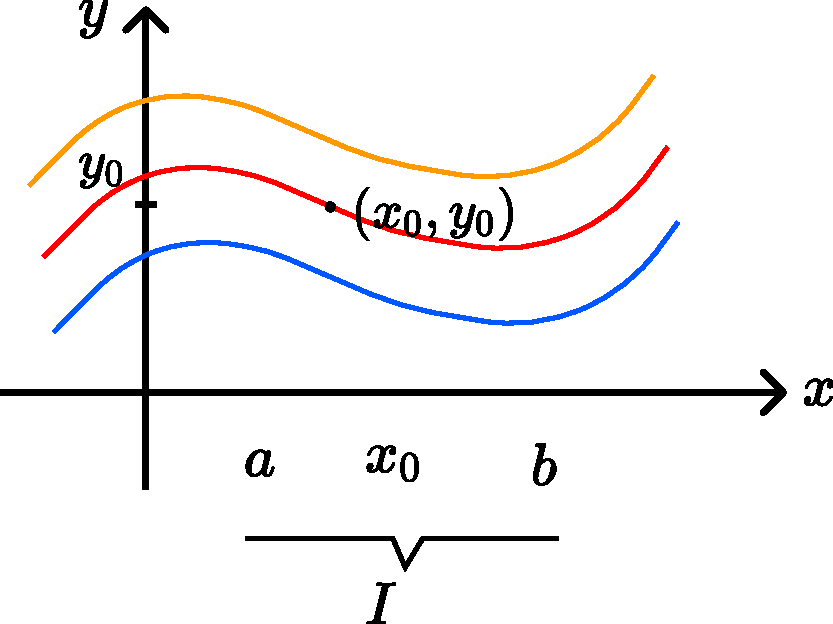
\includegraphics[width=0.5\textwidth]{ed2.pdf}
  \caption{Soluciones generales a la ecuación diferencial de segundo orden}
  \label{ed2}
\end{figure}

\begin{theorem}[Superposición]
    Considérese la ecuación diferencial homogénea asociada con \eqref{eq:ecuaciones_diferenciales_segundo_orden}:
    \begin{equation}
        a(x)y^{\prime\prime} + b(x)y^{\prime} + c(x)y= 0
        \label{eq:ecuaciones_diferenciales_segundo_orden_homogenea}
    \end{equation}
    Sean $y_1(x)$ y $y_2(x)$ soluciones de la ecuación
    La solución general es una combinación lineal de las soluciones individuales de una ecuación diferencial \eqref{eq:ecuaciones_diferenciales_segundo_orden_homogenea} en algún intervalo $I$. Entonces la combinación lineal 
    \begin{equation}
        y(x) = c_1y_1(x) + c_2y_2(x)
    \end{equation}
    Donde $c_1$ y $c_2$ son constantes también es solución de la ecuación diferencial \eqref{eq:ecuaciones_diferenciales_segundo_orden_homogenea} en el intervalo $I$.
\end{theorem}
Base canónica:
\begin{equation}
    a_{\R^2} = \left\{ e_1,e_2 \right\} = \left\{ (1,0), (0,1) \right\}
\end{equation}
$\R^2$ (No normal) sea $\gamma$ la nueva base. $\gamma= \left\{ (-1,2), (2,1) \right\}$
\begin{align*}
    &\gamma_1\cdot \gamma_2 = ( - 1,2)\cdot (2,1) = 0\\
    &(2, - 4) = c_1(- 1,2) + c_2(2,1)\\
    &2 =- c_1 + 2c_2\land - 4 = 2c_1 + c_2\\
    &c_1 = - 2\land c_2 = 0\\
    &(2, - 4) =- 2( - 1,2) + 0(2,1)
\end{align*}
\begin{definition}[Conjunto de funciones]
    Se dice que un conjunto de funciones $f_1$ y $f_2$ es \textbf{linealmente dependiente} en el intervalo $I$ si existen constantes $c_1$ y $c_2$ no todas cero, tales que:
    \begin{equation}
        c_1 + f_1(x) + c_2f_2(x) = \bar{0}\, \forall x\in I
    \end{equation}
    Si el conjunto de funciones no es linealmente dependiente en el intervalo $I$, se dice que es \textbf{Linealmente independiente}
\end{definition}

\begin{definition}
    Suponga que las funciones $f_1$ y $f_2$ tienen al menos $(n-1)$ derivadas en el intervalo $I$, entonces el determinante: 
    \begin{equation}
        W\left[ f_1,f_2 \right] = \det\begin{bmatrix}
            &f_1 &f_2  \\
            &f_1^{\prime}&f_2^{\prime}  
        \end{bmatrix}
    \end{equation}
Se le llama Wronstiano de las funciones $f_1$ y $f_2$
\end{definition}

\begin{theorem}
    Sean $y_1$ y $y_2$ dos soluciones de la ecuación diferencial \eqref{eq:ecuaciones_diferenciales_segundo_orden_homogenea} en el intervalo $I$. El conjunto formado por las soluciones $y_1$ y $y_2$ son linealmente independientes en $I$ sí y sólo sí $W[y_1,y_2]\neq 0\forall x\in I$.
\end{theorem}

\begin{definition}[Conjunto fundamental de soluciones]
    Es cualquier conjunto $\left\{y_1,y_2\right\}$ de dos soluciones linealmente independientes de la ecuación diferencial homogénea de segundo órden (2) en un intervalo I.
\end{definition}

\begin{theorem}[Existencia del conjunto fundamental de soluciones]
    Existe un conjunto fundamental de soluciones para la ecuación diferencial lineal homogénea de segundo orden (2) en el intervalo I.
\end{theorem}
\begin{theorem}
    Sea $\left\{y_1,y_2\right\}$ un conjunto fundamental de soluciones de la ecuación diferencial lineal homogénea de segundo orden (2) en el intervalo I. Entonces la solución general de la ecuación (2) en el intervalo I es:
    \begin{equation}
        y(x) = c_1y_1(x) +c_2y_2(x)
    \end{equation}
    Donde $c_1$ y $c_2$ son constantes arbitrarias
\end{theorem}

\section{Ecuación diferencial lineal homogénea con coeficientes constantes}
Considérese la ecuación diferencial: $1_2y^{\prime\prime}+a_1y^{\prime}(x)+a_0y(x)=0$
donde $a_2,a_1,a_0$ son constantes, $a_2\neq 0$. Se supondrá que la solución tiene la forma:
\begin{equation*}
    y(x) = e^{\lambda x}
\end{equation*}
Si es solución, entonces:
\begin{align*}
    a_2\cdot \lambda^2 e^{\lambda x} + a_1\cdot \lambda e^{\lambda x} + a_0 = 0\\
    e^{\lambda x}\left(a_2\lambda^2 + a_1\lambda + a_0\right) = 0
\end{align*}
Luego $e^{\lambda x}=0$ o $a_1\lambda^2+a_1\lambda^2+a_1\lambda^2+a_1\lambda+a_0=0$
pero $e^{\lambda x}\neq 0\forall \lambda$ y $\forall x$ por lo tanto $a_2\lambda^2+a_1\lambda+a_0=0$ es una ecuación algebraica la cual puede resolverse para $\lambda$ usando la fórmula general, entonces:
\begin{equation*}
    \lambda = \frac{ - a_1 \pm \sqrt{a_1^2 - a}_2a_0}{2a_2}
\end{equation*}
Se observan tres casos:
\begin{align*}
    \text{Caso 1: } a_1^2 - 4a_2a_0 > 0 \text{Caso de raíces reales y distintas}\\
    \implies \lambda_1 = \frac{ - a_1 + \sqrt{a_1^2 - 4a_2a_0}}{2a_2}; \lambda_2 = \frac{ - 1 - \sqrt{a_1^2 - 4a_2a_0}}{2a_2}
\end{align*}
Luego quiere decir que la solución diferencial tiene por soluciones a:
\begin{align*}
    y_1(x) = e^{\frac{ a_1 + \sqrt{a_1^2 - 4a_2a_0}}{2a_2}\cdot x}\\
    y_2(x) = e^{\frac{ a_1 - \sqrt{a_1^2 - 4a_2a_0}}{2a_2}\cdot x}
\end{align*}
Ya se tienen dos soluciones de la ecuación diferencial para el caso en el que $a_1^2-4a_2a_0>0$, ahora se tiene que verificar que $y_1,y_2$ son linealmente independientes, para ello se empleará el criterio de Wronskiano, es decir:
\begin{align*}
    &W\left[ y_1,y_2 \right] \det \begin{bmatrix}
        &e^{\frac{ - a_1 + \sqrt{a_1^2 - 4a_2a_0}}{2a_2}x}& e^{\frac{ - a_1 - \sqrt{a_1^2 - 4a_2a_0}}{2a_2}x}\\ 
        &\frac{ - a_1 + \sqrt{a_1^2 - 4a_2a_0}}{2a_2}e^{\frac{ - a_1 + \sqrt{a_1^2 - 4a_2a_0}}{2a_2}x}&\frac{ - a_1 - \sqrt{a_1^2 - 4a_2a_0}}{2a_2}e^{\frac{ - a_1 - \sqrt{a_1^2 - 4a_2a_0}}{2a_2}x}
    \end{bmatrix} =\\
    &=\frac{ - a_1 - \sqrt{a_1^2 - 4a_2a_0}}{2a_2}e^{\frac{ - a_1 + \sqrt{a_1^2 - 4a_2a_0}}{2a_2}x}\cdot e^{\frac{ - a_1 - \sqrt{a_1^2 - 4a_2a_0}}{2a_2}x} -\cdots\\
    &\cdots \frac{ - a_1 + \sqrt{a_1^2 - 4a_2a_0}}{2a_2}e^{\frac{ - a_1 + \sqrt{a_1^2 - 4a_2a_0}}{2a_2}x}\cdot e^{\frac{ - a_1 - \sqrt{a_1^2 - 4a_2a_0}}{2a_2}x}
\end{align*}
y se simplifica
\begin{align*}
    &=\frac{ - a_1 - \sqrt{a_1^2 - 4a_2a_0}}{2a_2}e^{ -\frac{a_1}{a_2}x} -\frac{ - a_1 + \sqrt{a_1^2 - 4a_2a_0}}{2a_2}e^{ -\frac{a_1}{a_2}x}\\
    &= e^{ -\frac{a_1}{a_2}x}\left[\frac{ a_1 - \sqrt{a_1^2 - 4a_2a_0} + a_1 - \sqrt{a_1^2 -4a_2a_0}}{2a_2}\right]\\
    &=e^{ -\frac{a_1}{a_2}x}\left[\frac{ - \sqrt{a_1^2 - 4a_2a_0}}{a_2}\right]\neq 0
\end{align*}
Las soluciones $y_1$ y $y_2$ son linealmente independientes, lo cual implica que forman un conjunto fundamental de soluciones para la ecuación diferencial y la solución general será una combinación lineal de ellas:
\begin{align*}
    y(x) = c_1e^{\frac{ -a_1 + \sqrt{a_1^2 - 4a_2a_0}}{2a_2}x} + c_2 e^{\frac{ -a_1 - \sqrt{a_1^2 - 4a_2a_0}}{2a_2}x}
\end{align*}

\begin{definition}[Fórmula de De Moivre]
    Afirma que para cualquier número complejo (y en particular, para cualquier número real) $x$ y para cualquier $n\in \mathbb{Z}$ se verifica que
    \begin{equation}
        \left(\cos{x} + i \sin{x}\right)^n = \cos{nx} + i \sin{nx}
    \end{equation}
\end{definition}
\begin{theorem}[Fórmula de Euler]
    para todo número real $x$, que representa un ángulo en el plano complejo. Aquí, $e$ es la base del logaritmo natural, $i$ es la unidad imaginaria, $\sin{x}$ y $\cos{x}$ son las funciones trigonométricas seno y coseno.
    \begin{align}
        &e^{ix} = \cos{x} + i \sin{x} \\
        &e^{ - ix} = \cos{x} - i \sin{x} \\
    \end{align}
\end{theorem}

Caso dos: $a_1^2-4a_2a_0=0$ Caso de raíces reales y repetidas.

Se observa entonces que 
\begin{align*}
    \lambda_1 = \frac{-a_1 + \sqrt{a}}{2a_2}&&\lambda_2 = \frac{-a_1 -\sqrt{a}}{2a_2} 
\end{align*}
Esto implica que no hay dos soluciones linealmente independientes de la ecuación diferencial, por lo tanto se tiene que buscar una segunda solución que sea linealmente independiente. Dicha solución se encuentra de la siguiente forma:
\begin{theorem}
    Si $y_1(x)$ es solución de la ecuación diferencial $a_2y^{\prime\prime}+a_1y9a_0y=0$ implica una segunda solución de $y_2(x)$ con $y_1(x)$ será:
    \begin{equation}
        y_2(x) = \int \frac{e^{ -\int \frac{a_1}{a_2}\,dx}}{\left(y_1(x)\right)^2}\,dx
    \end{equation}
\end{theorem}

Aplicando el teorema anterior al caso de la raíz real repetida, se obtendría lo siguiente:
\begin{align*}
    y_2(x) = e^{ -\frac{a_1}{2a_2}}\int \frac{e^{ -\frac{a_1}{a_2}x}}{e^{ -\frac{a_1}{a_2}x}}\,dx\\
    y_2(x) = e^{ -\frac{a_1}{2a_2}}\int\,dx =y_2(x) = e^{ -\frac{a_1}{2a_2}x}\cdot x
\end{align*}
Como el teorema especifica que $y_2(x)$ es $l_1$ de $y_1(x)$ la solución general de la ecuación diferencial para el caso de raíces reales repetidas sería:
\begin{equation}
    y(x) = C_1 e^{ -\frac{a_1}{2a_2}x} + C_2 e^{ -\frac{a_1}{2a_2}x}
\end{equation}

Caso 3 $a_1^2-4a_2a_0<0$ caso para raíces complejas:
\begin{equation*}
    \lambda = \frac{ a_1 + \sqrt{a_1^2 -4a_2a_0}}{2a_2} = \frac{ - a_1 + \sqrt{a_1^2 -4a_2a_0}i}{2a_2}
\end{equation*}
Un número complejo es de la forma: $Z=\alpha +i\beta$
donde $\alpha$ es la parte real y $\beta$ es la parte imaginaria de Z.
\subsubsection{Álgebra de números complejos}

Sean $Z_1$ y $Z_2\in \mathbb{C} $ se define las siguientes operaciones:

\textbf{Suma}
\begin{equation}
    Z_1 + Z_2 = \left(\alpha_1 +\beta_{1}i\right) +\left(\alpha_2 +\beta_2i\right) =\left(\alpha_1 +\alpha_2 \right) +\left(\beta_1+\beta_{2}\right)i
\end{equation}

\textbf{Producto}
\begin{equation}
    Z_1 \cdot Z_2 = \left(\alpha_1 +\beta_{1}i\right) \cdot \left(\alpha_2 +\beta_2i\right) = \left[\left( \alpha_1\cdot \alpha_2 \right) - \left(\beta_1\cdot\beta_2\right)\right] + \left[\alpha_1\beta_2 -\beta_1\alpha_2\right]i
\end{equation}

\textbf{Conjugado}
\begin{equation}
    \text{Si } Z=\alpha +\beta_i \implies \bar{Z}=\alpha -\beta_i
\end{equation}


\textbf{Inverso multiplicativo}

Sea $Z=\alpha+ \beta i$ ¿Cómo será $Z^{-1}$ tal que $Z\cdot Z^{-1}=1$?

\textit{ Sol. }
\begin{align*}
    \left(\alpha +\beta i\right) \cdot\left(\alpha +\beta i\right)^{ - 1} = 1 + 0i\\ 
    \left(\alpha +\beta i\right) \cdot \left(\delta +\gamma i\right) = 1+ 0i\\
    \left(\alpha\delta -\beta\gamma\right) +\left(\alpha\gamma-\beta\delta \right) = 1 + 0i\\ 
    \alpha\delta -\beta\gamma = 1\land \alpha\gamma +\beta\delta = 0\\
    \delta = \frac{1 +\beta\gamma}{\alpha}\implies \alpha\gamma +\beta \left(\frac{1 +\beta\gamma}{\alpha}\right) = 0\implies \alpha^2\gamma +\beta +\beta^2\gamma = 0\\
    \gamma = \left(\alpha^2 +\beta^2\right) =-\beta\implies \gamma = \frac{ -\beta}{\alpha^2 +\beta^2}\\
    \delta = \frac{1 +\beta\left(\frac{ -\beta}{\alpha^2 +\beta^2}\right)}{\alpha}\\
    \delta = \frac{\alpha}{\alpha^2 +\beta^2}
\end{align*}
Por lo tanto el inverso multiplicativo de $Z$ es:
\begin{equation}
    Z^{\prime} = \frac{\alpha}{\alpha^2 +\beta^2} -\frac{\beta}{\alpha^2 +\beta^2}i
\end{equation}

\textbf{Cociente}
Sean $Z_1$ y $Z_2\in \mathbb{C} $ se define la siguiente operación:
\begin{equation}
    \frac{Z_1}{Z_2} = Z_1\cdot Z_2^{ - 1}
\end{equation}
al final, el cociente resulta ser un producto

\textbf{Módulo}

Sea $Z=a+bi\in \mathbb{C}$ se define el módulo $Z$ como:
\begin{equation}
    \left\lvert Z\right\rvert = \sqrt{\alpha^2 +\beta^2}
\end{equation}

El módulo es la normal de $\mathbb{C}$

\subsubsection{Forma Polar}

Sean $r$ y $\theta$ coordenadas polares del punto $\left(\alpha, \beta \right)$
correspondiente a un número complejo $\mathbb{Z}$ no nulo $\mathbb{Z}=\alpha+\beta i$

\begin{figure}[h!]
\centering
  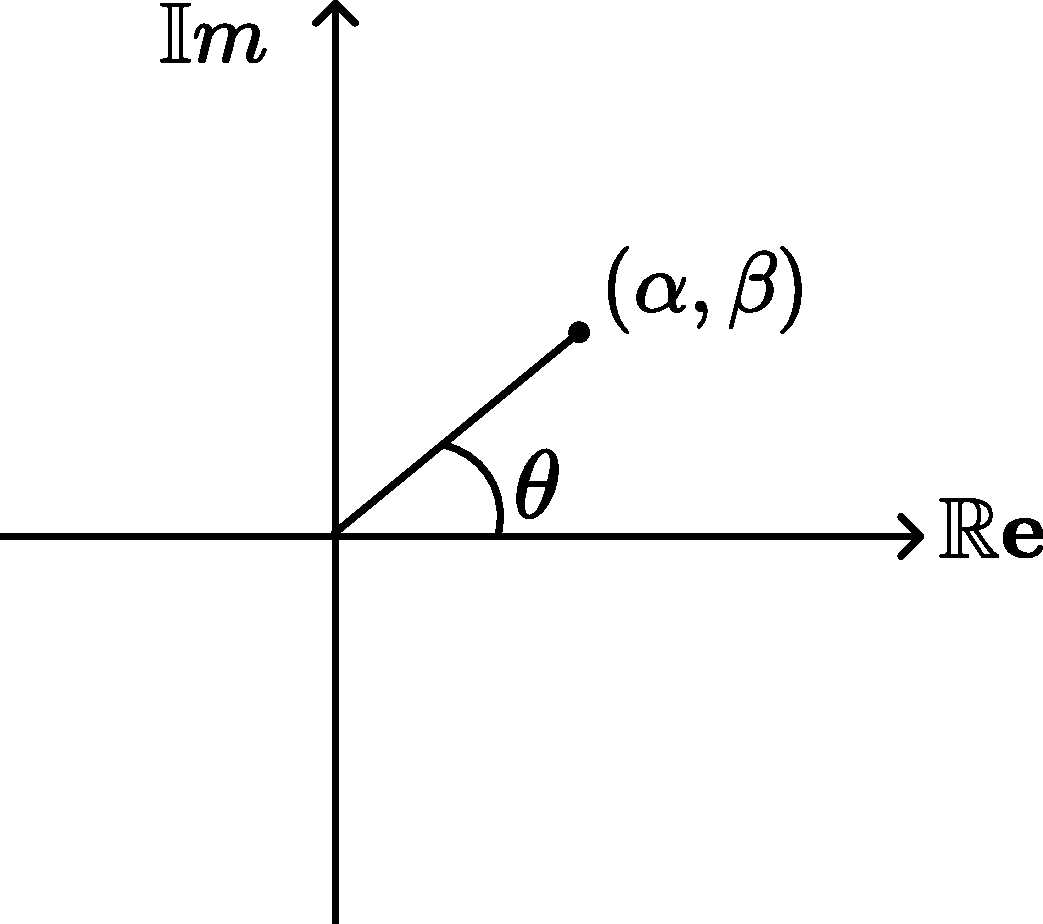
\includegraphics[width=0.5\textwidth]{ed3.pdf}
  \caption{Plano polar}
  \label{ed3}
\end{figure}
\begin{example}
    Escribir el número $z=1-i$ en la forma polar
\end{example}

\textit{ Sol. }
\begin{align*}
    &\alpha = \left\lvert z \right\rvert \cos{(\theta)}\\
    &\beta = \left\lvert z \right\rvert \sin{(\theta)} \\
    &z = \left\lvert z \right\rvert \cos{(\theta)}+\left\lvert z\right\rvert \sin{(\theta)}i
\end{align*}
La expresión simplificada será:
\begin{equation}
    z =\left\lvert z\right\rvert \left(\cos{(\theta)} + \sin{\theta}i\right) 
\end{equation}
forma polar del número $z=1-i$ en la forma polar.

El módulo de $z\left\lvert z\right\rvert = \sqrt{1^2+(-1)^2}=\sqrt{2}$
\begin{align*}
    &\alpha = \left\lvert z \right\rvert \cos{(\theta)} \implies 1 = \sqrt{2}\cos{\theta}\implies \frac{1}{\sqrt{2}} = \cos{(\theta)}  \\
    &\cos{(\theta)} = \frac{\sqrt{2}}{2}\implies \theta = \arccos{\left(\frac{\sqrt{2}}{2} \right)} = \frac{\pi}{4}\\
    &\beta = \left\lvert z\right\rvert \sin{(\theta)}\implies - 1 = \sqrt{2} \sin{(\theta)}\implies - \frac{1}{\sqrt{2}} = \cos{\theta}\\
    &\implies{(\theta)} = \frac{ -\sqrt{2}}{2}\Longleftrightarrow \theta = \frac{1}{4}\pi\left(8n -1\right) n \in \mathbb{Z}\\
    &n = 0\implies \theta = - \frac{\pi}{4}\\
    &n = 1\implies \theta = \frac{7\pi}{4}\\
    &\frac{\beta}{\alpha} = \frac{\left\lvert z\right\rvert \sin{(\theta)} }{\left\lvert z\right\rvert \cos{(\theta)}}\Longleftrightarrow \theta = \pi\left(n - \frac{1}{2}\right)n\in \mathbb{Z}\\
    &\frac{\beta}{\alpha} = \tan{(\theta)}\implies \theta = \arctan{\left(\frac{\beta}{\alpha}\right)}\Longleftrightarrow \theta\neq \pi\left(n - \frac{1}{2}\right)n\in \mathbb{Z}
\end{align*}
Retornando al ejemplo donde $\alpha=1$ y $\beta=-1$
\begin{equation*}
    \theta=- \pi/4, \frac{3\pi}{4}, \frac{7\pi}{4}
\end{equation*}
Por lo tanto la expresión polar para $z=1-i$
\begin{equation*}
    z = \sqrt{2}\left(\cos{\left( - \frac{\pi}{4}\right)} + i\sin{\left( -\frac{\pi}{4}\right)}  \right)
\end{equation*}
Otra forma de expresarlo puede ser:
\begin{equation*}
    z = \sqrt{z}\left(\cos{\left( - \frac{11\pi}{4}\right)} + i \sin{\left(\frac{11\pi}{4}\right)} \right)
\end{equation*}
En general cualquier número de la forma $z= \alpha+\beta i$ puede expresarse en forma polar
como:
\begin{equation}
    z =\left\lvert z\right\rvert \left(\cos{\left(\theta + n\pi\right)} + i \sin{\left(\theta + 2n\pi\right)} \right)
\end{equation}
Donde $\tan{(\theta)}= \frac{\beta}{\alpha}$
\begin{notation}
    $\theta=arg(z)$
\end{notation}

\subsection{Forma exponencial}

En ocasiones, es conveniente es escribir $e^{i\theta}$ o $exp(i\theta)$ en su forma polar:
\begin{equation*}
    z =\left\lvert z\right\rvert \left(\cos{(\theta)} + i \sin{(\theta)} \right)
\end{equation*}
¿Cómo se expresaría $e^z$?

se expresa como:
\begin{align*}
    &e^z = e^{\alpha + \beta i} = e{\alpha}\cdot e^{\pi}\\
    &e^z = e^{\left\lvert z\right\rvert\left(\cos{(\theta)} + i \sin{(\theta)} \right)} = e^{\left\lvert z\right\rvert}\cdot e^{\left(\cos{(\theta)} + i \sin{(\theta)} \right)}\\
    &e^z = e^{\left\lvert z\right\rvert}\cdot e^{\cos{(\theta)}}\cdot e^{i \sin{(\theta)}}\\
    &e^{i\theta} = \cos{(\theta)} + i \sin{(\theta)}\text{ Formula de Euler}\\
    &\left(e^{i\theta}\right)^n = \cos{(n\theta)} + i \sin{(n\theta)} \text{ Formula de De Moivre}
\end{align*}   
Para el caso $z=\alpha+\beta i$ la fórmula de Euler se transforma en lo siguiente:
\begin{equation}
    e^{\alpha + i\beta} = e^{\alpha}\cdot e^{i\beta} = e^{\alpha}\cdot \left(\cos{\beta} + i\sin{(\beta)} \right)
\end{equation}

¿Cómo sería $\left(e^{\alpha+i\beta}\right)^n$?
\begin{align*}
    \left(e^{\alpha+i\beta}\right)^n = \left(e^{\alpha}\cdot e^{i\beta}\right)^n =\left(e^{\alpha}\right)^n\cdot\left(e^{i\beta}\right)^n
\end{align*}
\begin{equation}
    \left(e^{\alpha + i\beta}\right)^n = e^{n\alpha}\cdot\left(\cos{(n\beta)} + i\sin{(n\beta)}  \right)
\end{equation}
Y para finalizar, 
\begin{align*}
    &\sin{(z)} = \frac{e^{iz} - e^{ - iz}}{2i} && \cos{(z)} = \frac{e^{iz} + e^{ -iz}}{2} 
\end{align*}
Como el discriminante $\Delta = a_1^2-4a_2a_0< 0$ esto da orígen a que la solución de la ecuación característica para calcular el valor de $\lambda$ sea un número complejo, entonces:
\begin{align*}
    &\lambda = \frac{ -a_1 \pm \sqrt{a_1^2 -4a_2 a_0}}{2a_2}\\
    &\lambda = \frac{ -a_1 \pm \sqrt{a_1^2 -4a_2 a_0}i}{2a_2}\\
    &\alpha =\frac{ -a}{2a_2}\quad \beta = \frac{\sqrt{a_1^2 -4a_2a_0}}{2a_2}\\
    &\lambda = \alpha \pm \beta i
\end{align*}
Por lo tanto las soluciones linealmente independientes quedarían como:

\begin{align*}
    &y(x) c_1 e^{\lambda_1x} + c_2 e^{\lambda_2x}\\
    &y(x) =c_1e^{\left(\alpha - \beta i\right) x} + c_2e^{\left(\alpha + \beta i\right) x}\\
    &y(x) = c_1e^{\alpha x}\left(\cos{(\beta x)} + i \sin{(\beta x)}  \right) + c_2e^{\alpha x}\left(\cos{(\beta x)} - i \sin{(\beta x)}  \right)\\
    &y(x) = c_1e^{\alpha x}\cos{(\beta x)} + c_1e^{\alpha x}i\sin{(\beta x)} + c_2e^{\alpha x}\cos{(\beta x)} - c_2e^{\alpha x}i\sin{(\beta x)}\\
    &y(x) = \left(c_1 + c_2\right)e^{\alpha x}\cos{(\beta x)} + \left(c_1 - c_2\right)  
\end{align*}
Definiendo a $k_1= c_1+c_2$ y $k_2=c_1-c_2$ de tal manera que la solución se forma con las partes real e imaginaria:
\begin{align*}
    &y(x) =k_1e^{\alpha x}\cos{(\beta x)} + k_2e^{\alpha x}i\sin{(\beta x)}\\
    &y(x) = e^{\alpha x}\left(k_1\cos{(\beta x)} + k_2 \sin{(\beta x)}  \right)
\end{align*}
Es la solución a la ecuación diferencial lineal de segundo orden con coeficientes constantes homogénea. (Caso raíces complejas)

\begin{example}
    Resuelva las siguientes ecuaciones diferenciales:
    \begin{equation*}
        y^{\prime\prime} + 3y^{\prime} - 10 =0
    \end{equation*}
\end{example}

\textit{ Sol. }

Se propone como solución una función de la forma $y(x)=e^{\lambda x}$; $\lambda$ es un número desconocido
\begin{align*}
    &y^{\prime}(x) = \lambda e^{\lambda x},\, y^{\prime\prime}(x) =\lambda^2e^{\lambda x}\\
    &\lambda^2 e^{\lambda x} + 3\lambda e^{\lambda x} - 10e^{\lambda x}= 0
\end{align*}
Factorizando $e^{\lambda x}$ se obtiene la ecuación característica para $\lambda$
\begin{align*}
    &\lambda \implies e^{\lambda x}\left(\lambda^2 + 3\lambda -10\right) = 0\\
    &\text{Como }e^{\lambda x} = 0\forall x
\end{align*}
Resolviendo $\lambda^2 + 3\lambda -10$, se obtiene $\lambda_1=-5$ y $\lambda_2=2$ por lo tanto las soluciones son:
\begin{align*}
    y_1(x) = e^{- 5x}&& y_2(x) = e^{2x}\\
\end{align*}
La solución a la ecuación diferencial homogénea 1 es:
\begin{equation}
    y(x) =c_1e^{ - 5x} +c_2e^{2x}
\end{equation}
Comprobación:
\begin{align*}
    &y^{\prime} =- 5c_1e^{ - 5x} + 2c_2e^{2x}\\
    &y^{\prime\prime} = 25c_1e^{ -5x} + 4c_2e^{2x}\\
\end{align*}
Sustituyendo en la ecuación diferencial se hace:
\begin{align*}
    25c_1e^{ -5x} + 4c_2e^{2x} - 15c_1e^{ -5x} + 6c_2e^{2x} -10c_1e^{ -5x} - 10c_2e^{2x} = 0
\end{align*}

\begin{example}
    \begin{equation*}
        4y^{\prime\prime} 12y^{\prime} + 9y = 0
    \end{equation*}
\end{example}

\textit{ Sol. }
La ecuación característica es $4\lambda^2-12\lambda+9=0$ así que $\lambda= \frac{3}{2}$
\begin{align*}
    y_1(x) = e^{\frac{3}{2}x}&& y_2(x) = xe^{\frac{3}{2}x}
\end{align*}
Finalmente la solución a la ecuación diferencial homogénea es:
\begin{equation*}
    y(x) = c_1e^{\frac{3}{2}x}+ c_2xe^{\frac{3}{2}x}
\end{equation*}

\begin{example}
    \begin{equation*}
        y^{\prime\prime} + 8y^{\prime} + 25 =0
    \end{equation*}
\end{example}

\textit{ Sol. }

La ecuación característica para $\lambda$
\begin{align*}
    \lambda = \frac{ - 8\pm \sqrt{ -25}}{2} = \begin{cases} \lambda_1 = \frac{- 8 + 6i}{2}\\\frac{- 8 - 6i}{2}
     \end{cases} 
\end{align*}

\begin{align*}
    \alpha =- 4\land \beta = 3
\end{align*}
Las soluciones son:
\begin{align*}
    y_1(x) = e^{- 4x} \cos{(3x)}\mid \mathbb{R}e && y_2(x) = e^{ - 4x}\sin{3x} \mid \mathbb{I}m
\end{align*}
De tal manera que la solución a la ecuación diferencial homogénea es:
\begin{equation*}
    y(x) = e^{ - 4x}\left(c_1\cos{(3x)} +c_2\sin{(3x)} \right)
\end{equation*}
\section{Solución de ecuaciones diferenciales con coeficientes con constantes No homogéneas}

Se pretende resolver la ecuación diferencial:
\begin{equation}
    a_2 y^{\prime\prime} + a_1y^{\prime} + a_0y = f(x)
    \label{eq:ecuaciondiferencial1}
\end{equation}
Tal que $f(x)$ es una función continua en el intervalo I (El intervalo de definición de $y(x)$). El método de coeficientes indeterminados tiene ciertas desventajas cuando el término de no homogeneidad es una función racional.

Así cuando el término de no homogeneidad tiene las siguientes formas, se propone una solución llamada particular a cada caso. Se debe de tomar en consideración que la solución general de la ecuación diferencial (\eqref{eq:ecuaciondiferencial1}) se compone de dos partes:
\begin{equation*}
    Y_g(x) = y_n(x) + y_p(x)
\end{equation*}
A reserva del resultado de $y_n(x)$ las propuestas de solución para $y_p(x)$ son:
\begin{table}[h!]\centering
    \begin{tabular}{@{}cc@{}}
    \toprule
    $f(x)$                                 & Forma $y_p(x)$                                            \\ \midrule
    Constante $\neq 0$                     & $A$                                                         \\
    $x$                                    & $Ax+B$                                                    \\
    $x^2$                                  & $Ax^2+B+C$                                                \\
    $\sin{(2x)}$                           & $A\cos{(2x)}+B\sin{(2x)}$                                 \\
    $e^{2x}$                               & $Ae^{2x}$                                                 \\
    $x^2e^{2x}$                            & $\left(Ax^2 + Bx + C\right)e^{2x}$                        \\
    \multicolumn{1}{l}{$e^{2x}\sin{(2x)}$} & \multicolumn{1}{l}{$Ae^{2x}\cos{(2x)} + Be^{2x}\sin{2x}$} \\ \bottomrule
    \end{tabular}
    \caption{Tabla de soluciones particulares de ecuaciones diferenciales}
    \label{tabed1}
\end{table}

\begin{example}
    Resolver la ecuación diferencial 
    \begin{equation*}
        y^{\prime\prime} + 3y^{\prime} + 2y = 3x^2 - x +
    \end{equation*}
\end{example}

\textit{ Sol. }

Siempre se resuelve la ecuación diferencial homogénea asociada con la ecuación diferencial dada:
\begin{equation*}
    y^{\prime\prime} + 3y^{\prime} + 2y = 0
\end{equation*}
\begin{align*}
    &y_1(x) = e^{-2x}&& y_2(x) = e^{-x}\\
    &\therefore y_n(x) = c_1e^{ - 2x} +c_2e^{ - x}
\end{align*}
Se propone una solución particular de la forma $y_p(x)=Ax^2+Bx+C$

Ahora se calculan $y^{\prime}_p(x)$ y $y_p^{\prime\prime}(x)$, sustituyendo en la primera ecuación:
\begin{align*}
    &y^{\prime}(x) = Ax + B\\
    &y^{\prime\prime}(x) = 2A\\
    &2A + 3\left(2Ax + B\right) + 2\left(Ax^2 Bx + C\right) = 3x^2 - x + 1
\end{align*}
Simplificando el lado izquierdo de la igualdad:
\begin{align*}
    &2A + Ax + 3B + 2Ax^2 + 2Bx + 2C = 3x^2 - x + 1\\
    &2Ax^2 + \left(6A + 2B\right)x +\left(2A + B + 2C\right) = 3x^2 - x + 1\\
    &2A = 3\land 6A + 2B =- 1\land 2A + 3B + 2C = 1\\
    &A = \frac{3}{2}\quad B =- 5\quad C = \frac{13}{2}
\end{align*}
Por lo tanto la solución particular $y_p(x)= \frac{3}{2}x^2-5x+\frac{13}{2}$
La solución general:
\begin{equation*}
    Y_g(x) =c_1e^{ -2x} +c_2e^{ - x} + \frac{3}{2}x^2 - 5x + \frac{13}{2}
\end{equation*}
\begin{example}
    Resolver la ecuación diferencial 
    \begin{equation*}
        y^{\prime\prime} + 4y^{\prime} + 4y = e^{ 2x}
    \end{equation*}
\end{example}
\textit{ Sol. }
El resultado de la ecuación diferencial homogénea asociada con la ecuación dada es:
\begin{equation*}
    y^{\prime\prime} 4y^{\prime} + y =0
\end{equation*}
Cuya solución es:
\begin{equation*}
    y_n(x) =c_1e^{ -2x} +c_2xe{ - 2x}
\end{equation*}
Ahora se propone una solución particular de la forma:
\begin{align*}
    &y_p(x) = Ae^{ -2x}\\
    &y^{\prime}(x) =- 2Ae^{ - 2x}; \quad y^{\prime\prime}(x) = 4Ae^{ - 2x}\\
    &4Ae^{ -2x} + 4\left( - 2Ae^{ -2x}\right) + 4Ae^{ - 2x} = e^{ 2x}\\
    &8Ae^{ - 2x} - 8Ae^{ - 2x} = e^{ 2x}\\
    &0 = e^{ 2x}\bot
\end{align*}
Al no funcionar la propuesta de solución particular $y_p(x)=Ae^{-2x}$ por ejemplo $y_p(x)=Axe^{-2x}$ tampoco funciona  porque en la $y_h(x)$ está el término $c_2xe^{-2x}$ por ello se propondrá que $y_p(x)=Ax^2e^{-2x}$
y se calculan las derivadas $y^{\prime}$, $y^{\prime\prime}$ para sustituirse en:
\begin{align*}
    &y^{\prime}(x) = 2Axe^{ - 2x} - 2Ax^2e^{ - 2x}\\
    &y^{\prime\prime}_p(x) = 2A^2e^{ - 2x} - 4Ae^{ - 2x} - 4Axe^{ - 2x} + 4Ax^2e^{ -2x}\\
    &y'^{\prime\prime\prime}(x) = 2Ae^{ - 2x} - 8Axe^{ - 2x} + 4Ax^2e^{ - 2x}\\
    &2Ae^{ - 2x} - 8Axe^{ - 2x} + 4Ax^2e^{ - 2x} + 8Axe^{ - 2x} - 8Ax^2e^{ - 2x} + 4Ax^2e^{ - 2x}= e^{ -2x}\\
    &2Ae^{ - 2x} = e^{ -2x}\implies A = \frac{1}{2}
\end{align*}
La solución particular o complementaria es:
\begin{equation*}
    y_p(x) = \frac{1}{2}x^2e^{ - 2x}
\end{equation*}
Finalmente la solución general de la ecuación es:
\begin{equation*}
    y_g(x) = c_1e^{ - 2x} + c_2xe^{ - 2x} + \frac{1}{2}x^2e^{ - 2x}
\end{equation*}
\begin{example}
    Resolver la ecuación diferencial 
    \begin{equation*}
        y^{\prime\prime} + 25y= 6 \sin{(x)} 
    \end{equation*}
\end{example}

\textit{ Sol. }

El polinomio a la ecuación diferencial asociada es decir:
\begin{equation*}
    y^{\prime\prime} + 25y = 0
\end{equation*}
cuyo polinomio característica es: $\lambda^2+25=0$, se tiene que $\lambda= \pm 5i$, por lo tanto $y_i(x)= \cos{(5x)}$
y $y_2(x)=\sin{(2x)}$, así la solución es:
\begin{equation*}
    y_n(x)= C_1 \cos{(5x)} C_2\sin{(5x)}
\end{equation*}
Se propone como solución particular:
\begin{align*}
    y_p(x) = A \cos{(x)} + B \sin{(x)}\\
    y_p^{\prime}(x) - A \sin{(x)} + B \cos{(x)} = 0\\
    y^{\prime\prime}_p (x) =- A \cos{(x)} + B \sin{(x)}
\end{align*}
Y se sustituye en la ecuación diferencial
\begin{align*}
    - A \cos{(x)} - B \sin{(x)} + 25A \cos{(x)} + 25B \sin{(x)} = 6 \sin{(x)}\\
    24A \cos{(x)} + 24B \sin{(x)} = 6 \sin{(x)}\\
    24A = 0\quad 24B = 6\\
    \therefore A = 0,\quad B = \frac{1}{4}
\end{align*}
Así la solución particular es:
\begin{equation*}
    y_p(x) = \frac{1}{4} \sin{(x)}
\end{equation*}
Finalmente la solución general es:
\begin{equation*}
    y_G(x) = A \cos{(5x)} + B \sin{(5x)} + \frac{1}{4} \sin{(x)}
\end{equation*}

\begin{example}
    Resolver la ecuación diferencial 
    \begin{equation*}
        y^{\prime\prime} - 5y^{\prime} = x - 2
    \end{equation*}
    $y(0)=0$, $y^{\prime}(0)=2$
\end{example}
\textit{ Sol. }

La solución de la ecuación diferencial homogénea
\begin{equation*}
    y_n(x) = c_1 +c_2 e^{5x}
\end{equation*}
La solución particular (Primera propuesta), será la siguiente:
\begin{equation*}
    y_p(x) = A_x+ B
\end{equation*}
No funcionaría porque hay dependencia lineal con un término de $y_h(x)$
Para eliminar la dependencia lineal, se multiplica $y_p$ por $x$ teniendo una segunda propuesta para $y_p$
\begin{equation*}
    y_p(x) = A_x + B_x
\end{equation*}
La cual ya es linealmente independiente de $y_h(x)$
\begin{align*}
    &y_p^{\prime}(x) = 2Ax + B\\
    &y_p^{\prime\prime}(x) = 2A
\end{align*}
Sustituyendo en la ecuación diferencial original:
\begin{align*}
    2A - 0Ax - 5B =x- 2\\
    - 10Ax +\left(2A - 5B\right) =x- 2\\
    -10A = 1\quad 2A - 5B =- 2\\
    A =-\frac{1}{10}\quad B =\frac{9}{25}
\end{align*}
Por lo tanto la solución particular es:
\begin{equation*}
    y_p(x) = -\frac{1}{10}x^2 + \frac{9}{25}x
\end{equation*}
Por lo tanto la solución general es:
\begin{equation*}
    y_G(x) =C_1 + C_2e^{5x} - \frac{1}{10}x^2 + \frac{9}{25}
\end{equation*}
Ahora se aplican las condiciones iniciales
\begin{align*}
    y_G(0) = C_1 + C_2 = 0\implies C_1 + C_2 = 0\\
    y^{\prime}_G(x) = 5C_2 e^{5x} - \frac{1}{5}x\\
    y^{\prime}_G(0) = 5C_2 =2\implies C_2 =\frac{2}{5}\\
    C_1+ \frac{2}{5} = 0\implies C_1 = -\frac{2}{5}
\end{align*}
La solución al P.V.I:
\begin{equation*}
    y(x) =- \frac{2}{5} + \frac{2}{5}e^{5x} - \frac{1}{10}x^2 + \frac{9}{25}x
\end{equation*}
\begin{example}
    \begin{equation*}
        y^{\prime\prime} + y = 8 \cos{(2x)} - 4 \sin{(x)}  
    \end{equation*}
\end{example}
\textit{ Sol. }
\begin{align*}
    \lambda^2 +1 = 0\implies \lambda = \pm i\\
    y_h(x) = c_1 \cos{(x)} + c_2 \sin{(x)}\\
    y_p(x) = A \cos{(2x)} + B \sin{(2x)} + C \cos{(x)} + D \sin{(x)}\\
    y_p(x) = A \cos{(2x)} + B \sin{(2x)} + Cx \cos{(x)} + Dx\sin{(x)}
\end{align*}

%%%%%%%%%%%%%%%%%%%%%%%%%%%%%%%

Al haber dependencia lineal en la segunda parte de la propuesta de la solución particular con la solución de la ecuación diferencial
para eliminar la dependencia lineal, entonces:
\begin{equation*}
        y_p(x) = A \cos{(2x)} + \sin{(2x)} + cx\cos{(x)} +Dx\sin{(x)}
\end{equation*}
Luego las derivadas de esta serán las siguientes:
\begin{align*}
    &y^{\prime}_p(x) =-2A \sin{(2x)} + 2B \cos{(2x)} +c \cos{(2x)} - cx \sin {(x)} + D \sin{(x)} + Dx \cos{(x)}\\ 
    &y^{\prime\prime}(x) =- 4A\cos{(2x)} - 4B\sin{(2x)} - 2c\sin{(2x)} - cx\cos{(x)} + 2D\cos{(2x)} - Dx\sin{(x)}
\end{align*}
Sustittuyendo en la ecuación diferencial, lo anterior para determinar los coeficientes.
\begin{equation*}
- 4A\cos{(2x)} - 4B\sin{(2x)} -2c\sin{(2x)} - Cx\cos{(x)} + 2D\cos{(x)} - Dx\sin{(x)} + Ax\cos{(2x)} + B\sin{(2x)} + cx\cos{(x)}+ Dx\sin{(x)} = 8\cos{(2x)} -4\sin{(x)}
\end{equation*}
Ahora se agrupan terminos:
\begin{equation*}
    - 3A\cos{(2x)} - 3B\sin{(2x)} - 2c\sin{(x)} + 2D\cos{(x)} = 8\cos{(2x)}- 4\sin{(x)}
\end{equation*}
Por lo tanto $-3A = 8$, $-3B=0$, $-2C=-4$, $2D=0$.
\begin{align*}
    &A =-\frac{8}{3}&& B = 0&&C = 2&&D = 0
\end{align*}
Por lo tanto la solución particular será:
\begin{equation*}
    y_p(x) =- \frac{8}{3}\cos{(2x)} + 2x \cos{(x)}  
\end{equation*}
Finalmente la solución general de la ecuación diferencial:
\begin{equation*}
    y_G(x) = C_1 \cos{(x)} +c_2 \sin{(x)} - \frac{8}{3} \cos{(2x)} +2x \cos{(x)}   
\end{equation*}

\begin{example}
    Resolver la ecuación $y^{3}+y^{\prime}=2-\sin{(x)}$
\end{example}

\textit{ Sol. }

Primero se resuleve la ecuación diferencial homogénea asociada a la ecuación diferencial:
\begin{align*}
    &y^{39}y^{\prime} =0\\
    &\left(\lambda^{3} +\lambda\right)e^{\lambda} = 0
\end{align*}
Por lo tanto $\lambda^3+\lambda=0 \implies \lambda\left(\lambda^2+1\right)=0$ de donde $\lambda_1=0$, y $\lambda^2+1=0\implies \lambda_2 \pm i$
Entonces la solución de la ecuación diferencial homogénea estará compuesta por:
\begin{align*}
    &y_1 = e^0&&y_2 =\cos{(x)}&&y_3 = \sin{(x)}  
\end{align*}
Donde la siguente ecuación es la solución:
\begin{equation*}
    y_h(x) c_1 +c_2 \cos{(x)} + c_3 \sin{(x)}  
\end{equation*}
Ahora se propone una solución particular para la ecuación diferencial:
\begin{align*}
    y^3 + y^{\prime}= 2- \sin{(x)}
\end{align*}
Sin embargo la propuesta $y_p=A+B\cos{(x)}+c\sin{(x)}$ es linealmente dependiente de $y_h(x)$; por lo tanto es necesario eliminar esa dependencia lineal, es decir que $y_p(x)$ tendrá la forma:
\begin{equation*}
    y_p(x)= Ax + Bx \cos{(x)} + Cx\sin{(x)} 
\end{equation*}
Ahora tanto $y^{\prime}$ como $y^3$ se sustituyen en la ecuación diferencial original y se obtiene lo siguiente:
\begin{align*}
    - 3B\cos{(x)} + Bx\sin{(x)} - 3C\sin{(x)} - Cx\cos{(x)} + A + B\cos{(x)} - Bx\sin{(x)} + Cx\sin{(x)} + Cx\cos{(x)} = 2- \sin{(x)}
\end{align*}
Simplificando:
\begin{align*}
    &A 2B\cos{(x)} -2C\sin{(x)} = 2 - \sin{(x)}\\
    &A = 2\quad - 2B = 0\implies B = 0\quad - 2C =- 1\implies C = \frac{1}{2}
\end{align*}
Finalmente la solución particular es:
\begin{align*}
    &y_p = 2x + \frac{1}{2}x \sin{(x)} \\
    &y_g(x) = c_1 + c_2 \cos{(x)} + c_3 \sin{(x)} +2x + \frac{1}{2}x \sin{(x)}
\end{align*}

\section{Método de variación de parámetros}	

Para resolver ecuaciones diferenciales, se pretende resolver una ecuación diferencial (segundo orden) de la forma:
\begin{equation}
    a_2(x) + y^{\prime\prime} + a_1(x)y^{\prime} + a_0y = g(x)
    \label{eq:diferencialmvp}
\end{equation}
Siempre y cuando $a_2(x)\neq 0\forall x\in$ (eq.\eqref{eq:diferencialmvp}) es posible simplificar en:
\begin{equation}
    y^{\prime\prime} + P(x)y^{\prime} + a(x)y = f(x)
    \label{eq:diferencialmvp2}
\end{equation}
\begin{align*}
    &Donde\, P(x) = \frac{a_1(x)}{a_2(x)};&&Q(x) = \frac{a_0(x)}{a_2(x)};&&f(x) = \frac{g(x)}{a_2(x)}
\end{align*}
El proceso de solución después de asegurarse que el coeficiente de $y^{\prime\prime}$ es el siguiente:

Resolver la ecuacion diferencial homogénea asociada con (eq. \eqref{eq:diferencialmvp2}). Es claro que e obtienen dos soluciones linealmente independientes a saber $y_1(x)$, $y_2(x)$

El siguiente paso es suponer qye hay una solución particular complementaria de la forma:
\begin{equation}
    y_p(x) = u_1(x)\cdot y_1(x) + u_2(x)\cdot y_2(x)
    \label{eq:diferencialmvp3}
\end{equation}
Así el problema se reduce a encontrar las funciones desconocidas $u_1(x)$ y $u_2(x)$.

Al ser la (eq. \eqref{eq:diferencialmvp3}) solución de (eq. \eqref{eq:diferencialmvp2}), deberá satisfacerla:
\begin{equation*}
    y^{\prime}_p(x) = u^{\prime}_1(x)y_1(x) + u_1(x)y^{\prime}_1(x) + u^{\prime}_2(x)y_2(x) + u_2(x)y^{\prime}_2(x)
\end{equation*}
Calculando una segunda derivada:
\begin{equation*}
    y^{\prime\prime}_p(x) = 
\end{equation*}
Y se sustituyen en $y_p(x)$,$y^{\prime}_p(x)$,$y^{\prime\prime}_p(x)$ en la ecuación diferencial (eq. \eqref{eq:diferencialmvp2}):
\begin{align*}
    &y^{\prime\prime}_p(x) + P(x)y^{\prime}_p(x) + Q(x)y_p(x) = f(x)\\
    &\left(u^{\prime\prime}_1(x)y_1(x) + u^{\prime}_1(x)y^{\prime}_1(x) + u^{\prime}_1(x)y^{\prime}_1(x) + u_1(x)y^{\prime\prime}_1(x) + u_2^{\prime\prime}(x)y_2(x) + u^{\prime}_2(x)y^{\prime}_2(x) + u_2^{\prime}(x)y^{\prime}_2(x) + u_2(x)y^{\prime\prime}_2(x)\right) + \dots 
    &+ P(x)\left(u_1^{\prime}(x)y_1 + u_1y_1(x)^{\prime} +u_2^{\prime}(x)y_2 + u_2y_2(x)^{\prime} \right) + Q(x)\left(u_1(x)y_1 + u_2(x)y_2\right) = f(x)
\end{align*}
Agrupando términos:
\begin{equation*}
    u_1(x)\left(y_1^{\prime\prime} + P(x)y^{\prime}_1 + Q(x)y_1 \right) + u_2(x)\left(y_2^{\prime\prime} + P(x)y^{\prime}_2 + Q(x)y_2 \right) + \dots = f(x)
\end{equation*}
Como $y_1$, $y_2$ son soluciones linealmente independientes de la ecuación diferencial homogénea es 0.
\begin{align*}
    &u^{\prime\prime}_1(x)y_1(x) + u^{\prime}_1(x)y^{\prime}_1(x) + u^{\prime}_1(x)y^{\prime}_1(x) +  u_2^{\prime\prime}(x)y_2(x) + u^{\prime}_2(x)y^{\prime}_2(x) + u_2^{\prime}(x)y^{\prime}_2(x)+ u_2^{\prime}(x)y^{\prime}_2(x) + P(x)\left((u_1^{\prime}(x)y_1+u_2^{\prime}(x)y_2 \right) = f(x)\\ 
    &\left[u_1^{\prime}(x)y_1(x)+u_2^{\prime}y_2(x)\right]^{\prime}+P(x)\left[u_1^{\prime}(x)y_1(x)+u_2^{\prime}(x)y_2(x)\right]+\left[u_1(x)^{\prime}+y^{\prime}_1(x)+u^{\prime}_2(x)y_2^{\prime}(x) \right] = f(x)
\end{align*}
Es necesario suponer lo siguiente:
\begin{align*}
    &u_1^{\prime}(x)y_1(x)+u_2^{\prime}(x)y_2(x) = 0\\
    &\implies u_1^{\prime}(x)y_1^{\prime}(x) + u_2^{\prime}(x)y_2^{\prime}(x) = f(x)
\end{align*}
Multiplicando la ecuación por $y_2(x)$ y al planteamiento se multiplica por $y_2^{\prime}(x)$
\begin{align*}
    &u_1^{\prime}(x)y_1(x)+u_2^{\prime}(x)y_2(x) = 0\\
    &\implies u_1^{\prime}(x)y_1^{\prime}(x)y_2(x) + u_2^{\prime}(x)y_2^{\prime}(x)y_2(x) = f(x)y_2(x)\\
    &u_1^{\prime}(x)\left[y_1(x)y_2^{\prime}(x) - y^{\prime}_1(x)y_2(x) \right] + u^{\prime}_2(x)\left[y_2(x)y_2^{\prime}(x) -y_2^{\prime}(x)y_2(x)\right] =-f(x)y_2(x)\\
    &u_1^{\prime}(x)\left[y_1(x)y_2^{\prime}(x) - y^{\prime}_1(x)y_2(x) \right] = -f(x)y_2(x)
\end{align*}
Recordando:
\begin{equation}
    W\left[y_1,y_2\right] = \det\begin{bmatrix}
        y_1(x) & y_2(x)\\
        y_1^{\prime}(x) & y^{\prime}_2(x)
    \end{bmatrix} = y_1(x)y_2^{\prime}(x) - y_1^{\prime}y_2(x)
\end{equation}
\begin{equation*}
    \therefore u_1^{\prime}(x)\cdot W\left[y_1,y_2\right] = - f(x)y_2(x)
\end{equation*}
Y debido a que $y_1,y_2$ son funciones conocidas:
\begin{align*}
    &u^{\prime}_1(x) =-\frac{f(x)y_2(x)}{W\left[y_1(x),y_2(x)\right]}\\
    &u_1(x) = -\int \frac{f(x)y_2(x)}{W\left[y_1(x),y_2(x)\right]}\,dx
\end{align*}
Realizando un procedimiento similar para determinar $u_2$ se llegará a la siguiente expresión:
\begin{equation*}
    u_2(x) = -\int \frac{f(x)y_1(x)}{W\left[y_1(x),y_2(x)\right]}\,dx
\end{equation*}
Recordando la forma de la solución particular se tendrá que:
\begin{equation*}
    y_p(x) = \left[ -\int u_1(x) = -\int \frac{f(x)y_2(x)}{W\left[y_1(x),y_2(x)\right]}\,dx\right] y_1(x) + \left[\int \frac{f(x)y_1(x)}{W\left[y_1(x),y_2(x)\right]}\,dx\right]y_2(x)
\end{equation*}
Así la solución general será:
\begin{equation*}
    y_G(x) = c_1y_1(x) + c_2y_2(x) +y_p(x)
\end{equation*}
\begin{example}
    Resolver la ecuación diferencial
    \begin{align*}
        &\frac{d^2y}{dt^2} +y = \tan{(t)} &&y(0) =1&& y^{\prime}(0) =1
    \end{align*}
\end{example}
\textit{ Sol. }

Se observa que la ecuación en el término $\ddot{y}$, su coeficiente es igual a uno. Así que se procede a resolver la ecuación diferencial homogénea asociada:
\begin{equation*}
    \ddot{y}+y=0
\end{equation*}
La ecuación característica asociada es:
\begin{equation*}
    \lambda^2 + 1 = 0
\end{equation*}
Las soluciones son:
\begin{align*}
    &y_1(x) = \cos{(t)}&&y_2(x) = \sin{(t)}\\
    &y_h(x) = c_1 \cos{(t)} + c_2 \sin{(t)} 
\end{align*}
Se determinan las funciones $u_1(x),u_2(t)$ tales que $y_p(t)=u_1(t)y_1(t)+u_2(t)y_2(t)$ que en cuyo caso son:
\begin{equation*}
    u_1(t) =-\int \frac{f(t)y_2(t)}{W\left[y_1(t),y_2(t)\right]}\,dt
\end{equation*}
Calculando $W\left[\cos{(t)},\sin{(t)}\right]$ se tiene:
\begin{align*}
    &\left[\cos{(t)},\sin{(t)}\right] = \det\begin{bmatrix}
        \cos{(t)} & \sin{(t)}\\
        -\sin{(t)} & \cos{(t)}
    \end{bmatrix}\\
    &\cos^2{(t)} +\sin^2{(t)}=1\\
    &u_1(t) =-\int \frac{\tan{(t)}\cdot \sin{(t)}}{1}\,dt\\
    &u_1(t) =-\int \frac{\sin^2{(t)}}{\cos{(t)} }\,dt = -\int \frac{1 -\cos^2{(t)} }{\cos{(t)}}\,dt\\
    &u_1(t) = -\int \sec{(t)} \,dt = +\int \cos{(t)}\,dt\\
    &u_1(t) = -\ln{\sec{(t)}+\tan {(t)}}+ \sin{(t)} k_1
\end{align*}
Determinando a $u_2(t)$
\begin{align*}
    &u_2(t) = -\int \frac{f(t)y_1(t)}{W\left[y_1(t),y_2(t)\right]}\,dt\\
    &u_2(t) = -\int \frac{\tan{(t)}\cos{(t)}}{1}\,dt
\end{align*}
Por lo tanto la solución particular será:
\begin{align*}
    &y_p(t) =\left[ -\ln{\sec{(t)} + \tan{(t)}} + \sin{(t)} + \sin{(t)} k_1 \right]\cos{(t)} + \left(\cos{(t)}+ k_2 \right)\sin{(t)} \\
    &y_p(t)= c_1\cos{(t)} +c_2-\sin{(t)} -\ln{\sec{(t)} + \tan{(t)}}\cdot \cos{(t)} + \sin{(t)}\cos{(t)}+ k_1 \cos{(t)} -\cos{(t)}\sin{(t)} + k_2\sin{(t)}   
\end{align*}
Finalmente la solución general sería:
\begin{equation*}
    y_G(t) = c_1 \cos{(t)} + c_2 \sin{(t)} - \cos{(t)}\cdot\ln{\sec{(t)} + \tan{(t)}} 
\end{equation*}
%Aplicando las condiciones iniciales:
\begin{example}
    Resolver la ecuación diferencial $y^{\prime\prime}+3y^{\prime}+2y=\frac{1}{1+e^x}$
\end{example}

\textit{ Sol. }

Primer paso: verificar que el coeficiente de $y^{\prime\prime}$ (en este caso sea igual a 1), lo cual se cumple.

Segundo paso: Resolver la ecuación diferencial homogénea asociada con la ecuación diferencial original, hay que resolver: $y^{\prime\prime}+3y^{\prime}+2y=0$
donde $m_1=-1$ y $m_2=-2$ (Raíces de la ecuación característica) esto implicaría que $y_1(x)=e^{-x}$ y $y_2(x)=e^{-2x}$. Luego la solución de la ecuación diferencial homogénea es:
\begin{equation*}
    y_h(x)= c_1e^{- x}+c_2e^{-2x}
\end{equation*}

Tercer paso: Se determina una solución particular $y_p(x)$ de la forma:
\begin{equation*}
    y_p(x) = u_1(x)\cdot y_1(x)+ u_2(x) y_2(x)
\end{equation*}
Sin embargo, es necesario determinar un elemento más ``el Wronstiano''
\begin{equation*}
    W\left[y_1,y_2\right] = \det\begin{bmatrix}
        e^{ -x} & e^{ -2x}\\
        -e^{-x}&- 2e^{ -2x}
    \end{bmatrix} =-2e^{ -3x}+e^{ -3x}=-e^{ -3x}
\end{equation*}
Luego:
\begin{align*}
    &u_1(x)=\int \frac{-f(x)y_2(x)}{W\left[y_1,y_2\right]}\,dx=-\int\frac{\frac{1}{1 +e^x}\cdot e^{-2x}}{-e^{- 3x}}\,dx\\
    &u_1(x)=\int \frac{e^x}{1 +e^x}\,dx= \ln{1+ e^x}+ k_1\\
    &u_2(x)=\int \frac{f(x)y_1(x)}{W\left[y_1,y_2\right]}\,dx=-\int\frac{\frac{1}{1 +e^{ -x}}\cdot e^{ -3x}}{-e^{- 3x}}\,dx =\int\frac{e^{2x}}{1+ e^x}\,dx
\end{align*}
Para resolver la integral, se propone que $u=1+e^x\implies du=e^x\,dx$ entonces $u-1=e^x$: 

\begin{align*}
    \int\frac{u -1}{u}\,du = \int 1 + \frac{1}{u}\,du = u+\ln{(u)}+ k_2\\
    = 1+ e^x+\ln{(1+ e^x)} +k_2
\end{align*}
Poe lo tanto la solución particular es:
\begin{equation*}
    y_p(x) = e^{-x}\ln{(1+e^x)}+e^{-2x}+e{-x}+ e^{-2x}\ln{(1+ e^x)}
\end{equation*}
Finalmente la solución general es:
\begin{align*}
    &y_G(x)= c_1e^{-x}+c_2e^{-2x}+e^{-x}+e^{-x}\ln{(1+e^{x})}+e^{- 2x}\ln{(1+e^x)}\\
    &y_G(x)= c_1e^{-x}+c_2e^{-2x} +\ln{(1+e^{x})}\left[e^{- x}+e^{-2x}\right]
\end{align*}

\begin{example}
    Resolver la ecuación diferencial $y^{\prime\prime}-2y^{\prime}+y=\frac{e^x}{1+x^2}$
\end{example}

\textit{ Sol. }

La solución a la ecuación diferencial homogénea: $y_h(x)=c_1e^x+c_2xe^x$.
El Wronskiano $W\left[y_1,y_2\right]=e^{2x}$
\begin{equation*}
    u_1(x) = - \frac{1}{2}\ln{(1+ x^2)}
\end{equation*}
En tanto que:
\begin{align*}
    &u_2(x) = \int \frac{\frac{e^x}{1 x^2}\cdot e^x}{e^{2x}}\,dx\\ 
    &u_2(x)=\int \frac{dx}{1 +x^2}=\arctan{(x)} +k_2
\end{align*}
Por lo tanto la solución particular será:
\begin{equation*}
    y_p(x) = -\frac{1}{2}e^x\ln{1 +x^2} xe^x\arctan{(x)}
\end{equation*}
Finalmente la solución general será:
\begin{equation*}
    y_G(x) = c_1e^x + c_2^xe^x -\frac{1}{2}e^x\ln{1 +x^2} xe^x\arctan{(x)}
\end{equation*}

%%%%%%%%%%%%%%%%%%%%%%%%%
%%%%%%%%%%%%%%%%%%%%%%%
%%%%%%%%%%%%%%%%%%%%%%%%
%%%%%%%%%%%%%%%%%%
%%%%%%%%%%%%%%%%%%%%%%%%%%%
%%%%%%%%%%%%%%%%%%%%%%%%%%%%%%%%%%%%%


Calculando $\mathfrak{L}\left\{f^{\prime\prime}(t)\right\}= s^2F(S)-sf(0)-f^{\prime}(0)$

En general, la transformada de Laplace para una derivada de órden ``n''sería:
\begin{equation}
    \mathfrak{L}\left\{S^nF(S) S^{n -1}f(0)  \right\}
\end{equation}

\subsection{Transformada inversa}
$\mathfrak{L}\left\{1\right\}= \frac{1}{S}$ al aplicar el operador inverso a cada lado de la igualdad se obtiene:
\begin{equation}
    \mathfrak{L}\left\{\mathfrak{L}\left\{1\right\} \right\} = \mathfrak{L}^{- 1}\left\{\frac{1}{S}\right\}\implies 1 = \mathfrak{L}^{ -1}\left\{\frac{1}{S}\right\}
\end{equation}
\begin{equation}
    \mathfrak{L}\left\{t\right\} = \frac{1}{S^{2}}\implies t = \mathfrak{L}^{ -1}\left\{\frac{1}{S^2}\right\}
\end{equation}
Todas las propiedades de la integral son heredadas a la transformada de Laplace y de igual manera a la transformada inversa:
\begin{align}
    \mathfrak{L}\left\{kf(t)\right\} = k\mathfrak{L}\left\{f(t)\right\}\\
    \mathfrak{L}\left\{f(t)\pm g(t) \right\} = \mathfrak{L}\left\{f(t)\right\}\pm \mathfrak{L}\left\{g(t)\right\}
\end{align}
Y de forma  análoga para la transformada inversa.
\begin{example}
    Determinar $\mathfrak{L}^{-1}\left\{\frac{2}{S^4} \right\}$
\end{example}
\textit{ Sol. }

El caso general de la transformada directa de $\mathfrak{L}\left\{t^n\right\}= \frac{n!}{S^{n+1}}$
obsérvese que $\frac{2}{S^4}$ es algo de la forma $\frac{2}{S^{3+1}}$
\begin{align*}
    &\mathfrak{L}\left\{\frac{2}{S^4}\right\} = \mathfrak{L}^{- 1}\left\{\frac{3!}{3!}\cdot \frac{2}{S^{3 +1}}\right\} = \mathfrak{L}^{ -1}\left\{\frac{1}{3}\cdot \frac{3!}{S^{3 +1}}\right\}\\
    &= \frac{1}{3}\mathfrak{L}^{ -1}\left\{\frac{3!}{S^{3 +1}}\right\} = \frac{1}{3}t^3\\
    &\therefore \mathfrak{L}^{ -1}\left\{\frac{3}{S^4}\right\} = \frac{1}{3}t^3
\end{align*}

\begin{example}
    Calcular $\mathfrak{L}^{-1}\left\{\frac{1}{S^2+4}\right\}$
\end{example}
\textit{ Sol. }

La transformada directa $\mathfrak{L}\left\{\sin{(\omega t)}\right\}= \frac{\omega}{S^2+\omega^2}$
Ordenando la expresión en la transformada inversa:
\begin{align*}
    \mathfrak{L}^{ -1}\left\{\frac{1}{S^2 +4}\right\} = \mathfrak{L}^{- 1}\left\{\frac{1}{S^2 +2^2}\right\} = \mathfrak{L}^{ -1}\left\{\frac{1}{2}\cdot \frac{2}{S^2 +2^2}\right\}\\
    = \frac{1}{2}\mathfrak{L}^{ -1}\left\{\frac{2}{S^2 + 2^2}\right\} = \frac{1}{2} \sin{(2t)}\\
    \therefore \mathfrak{L}^{ -1}\left\{\frac{1}{S^2 +4}\right\} = \frac{1}{2} \sin{(2t)}  
\end{align*}

\begin{example}
    Determinar $\mathfrak{L}^{-1}\left\{\frac{S^2+6S+9}{S^3+5^2-10S+8}\right\}$
\end{example}
\textit{ Sol. }

Se intentará factorizar el denominador con la finalidad de aplicar el método de fracciones parciales.
\begin{align*}
    &g(S) = S^3 +S^2 - 10S +8\implies g(0)=8\\
    &g(1)= 0\implies S^3 S^2 - 10S + 8 \text{Puede ser dividido por }S-1\\
    &\frac{S-1}{S^3 +S^2 - 10S + 8} = S^2 + 2S - 8\implies (S -1)\left(S^2 + 2S - 8\right) = S^3 + S^2 -10S + 8
\end{align*}
Se intentará factorizar $S^2 + 2S - 8= \left(S+4\right)\left(S-2\right)$
Sustituyendo en el argumento de la transformada inversa tenemos:
\begin{align*}
    \mathfrak{L}^{ - 1} =\left\{\frac{S^2 +6S + 9}{S^3 +S^2 - 10S + 8}\right\} = \mathfrak{L}^{ -1}\left\{\frac{S^2 + 6S +9}{(S +4)(S -1)(S - 2)}\right\}
\end{align*}
Ahora se realizará una descomposición en fracciones simples del argumento de la transformada inversa
\begin{align*}
    &\frac{S^2 + 6S +9}{(S + 4)(S - 1)(S - 2)} = \frac{A}{S +4} + \frac{B}{S - 1} + \frac{C}{S - 2}\\
    &\frac{A(S - 1)(S - 2) + B(S + 4)(S - 2) + C(S + 4)(S - 1)}{(S + 4)(S - 1)(S - 2)} = \\
    &S^2 + 6S + 9 = A(S - 1)(S - 2) + B(S + 4)(S - 2) + C(S + 4)(S - 1)
\end{align*}
Sea $S=1\implies 1+6+9= B(5)(-1)\implies 16=-5B\implies B= -\frac{16}{5}$, sea $S=2$ entonces 4+12+9=C(6)(1)$\implies25=6C\implies C=\frac{25}{6}$
Si $S=-4\implies 16-24+9=A(-5)(-6)\implies 1=30A\implies A=\frac{1}{30}$
Obtenidos los valores de los coeficientes en las derivdaas parciales se tiene que:
\begin{equation*}
    \frac{S^2 + 6S +9}{(S + 4)(S - 1)(S - 2)} = \frac{\frac{1}{30}}{S +4} + \frac{-\frac{16}{5}}{S - 1} + \frac{\frac{25}{6}}{S - 2}
\end{equation*}
por lo tanto al aplicar la transformada inversa de Laplace, se obtiene:
\begin{align*}
    &\mathfrak{L}^{ -1}\left\{\frac{S^2 + 6S +9}{(S + 4)(S - 1)(S - 2)}\right\}= \mathfrak{L}^{ -1}\left\{\frac{\frac{1}{30}}{S +4}\right\} + \mathfrak{L}^{-1}\left\{\frac{ - \frac{16}{5}}{S - 1}\right\}\frac{-\frac{16}{5}}{S - 1} + \mathfrak{L}^{ -1}\left\{\frac{\frac{25}{6}}{S - 2}\right\}\\
    &= \frac{1}{30}e^{ - 4t} - \frac{16}{5}e^{t} + \frac{25}{6}e^{2t}0\\
\end{align*}

\begin{example}
    Aplicar el método de la transformada de Laplace para resolver la ecuación diferencial:
    \begin{equation*}
        \dot{y} - y= 1; y(0) =0
    \end{equation*}
\end{example}
\textit{ Sol. }

Se aplica la transformada de Laplace en ambos lados de la ecuación diferencial.
\begin{equation*}
    \mathfrak{L}\left\{\dot{y} -y\right\} =\mathfrak{L}\left\{1\right\}\implies \mathfrak{L}\left\{\dot{y}\right\}-\mathfrak{L}\left\{y\right\} = \mathfrak{L}\left\{1\right\}
\end{equation*}
La transofrmada de la primera derivada $\mathfrak{L}\left\{y^{\prime}\right\}=SF(s)-f(0)$

\begin{align*}
    &SF(S)- 0-F(S) = \frac{1}{S}\\
    &F(S)(S -1) = \frac{1}{S}\implies F(S)= \frac{1}{S(S -1)}\\
    &\mathfrak{L}^{ -1}\left\{F(S)\right\} \mathfrak{L}\left\{\frac{1}{S(S -1)}\right\}\implies y(t) = \mathfrak{L}\left\{1\right\}
\end{align*}
Se hace la descomposición en fracciones simples de la expresión:
\begin{equation*}
    \frac{1}{S(S -1)} = \frac{A}{S} + \frac{B}{S -1}\implies \frac{1}{S(S 1)} = \frac{AS -A + BS}{S(S -1)}\\
    \implies 1 = AS - A + BS\implies \begin{cases} A + B = 0\\
    - -A = 1\end{cases} 
\end{equation*}
Entonces $A=-1$ y $B=1$, esto conduce que $y(t) = - 1 +e^t$.

\subsection{Transformada de una función continua por tramos}

Se tiene que verificar la función dada por secciones sea continua, que la función dada por secciones tenga como dominio $[0,\infty)$,

\begin{example}
    Calcule $\mathfrak{L}\left\{f(t)\right\} $ si $f(t)=\begin{cases}
        &4\,si\, 0\leq t<2\\
        &0\,si\, t\geq 2
    \end{cases}$
\end{example}

\textit{ Sol. }

\begin{align*}
    &\mathfrak{L}\left\{f(t)\right\} = \int_0^{\infty}e^{ - St}f(t)\,dt = \int_0^2e^{ - St}_4\,dt +\int_2^{\infty} e^{ - St}0\,dt\\
    &= 4\int_0^2e^{ - St}_4\,dt = - \frac{4}{S}e^{- St}\mid_0^2 = - \frac{4}{S}\left(e^{ - 2S} - e^0\right)\\
    &= - \frac{4}{S}e^{- 2S} + \frac{4}{S}\quad S > 0
\end{align*}

\begin{example}
    Calcular la transformada de Laplace de la función
    \begin{equation*}
        f(t)=\begin{cases}
            &t\,si\, 0\leq t< 1\\ 
            &1\,si\, t\geq 1
        \end{cases}
    \end{equation*}
\end{example}

\textit{ Sol. }

Aplicando la definición de la transformada a la función $f(t)$ se obtiene 

\begin{align*}
    &\mathfrak{L}\left\{f(t)\right\} = \int_0^{\infty}e^{ - St}f(t)\,dt = \int_0^1e^{ - St}t\,dt +\int_1^{\infty} e^{ - St}1\,dt\\
    &\int_0^1 e^{ - St}t\,dt = - t\cdot \frac{1}{S}e^{- St}\mid_0^1 + \int_0^1 \frac{1}{S}e^{ -St}\,dt\\
    &= - \frac{t}{S}e^{ - St}\mid_0^1 - \frac{1}{S^2}e^{ - St}\mid_0^1 = \left(- \frac{1}{S} - 0\right) - \frac{1}{S^2}\left(e^{ - S} - e^0\right)\\
    &=- \frac{1}{S}e^{ - S} - \frac{1}{S^2}e^{ - S} + \frac{1}{S}e^{ - S} =- \frac{1}{S^2}e^{ - S}\\
    &\lim_{b\to \infty}\int_1^b e^{ - St}\,dt =\lim_{b\to \infty} \left[- \frac{1}{S}e^{ - St}\right]_1^b =\\
    &\lim_{b\to \infty} - \frac{1}{S}\left(e^{ - Sb} e^{ - S}\right) = \frac{1}{S}e^{ - S} - \frac{1}{S^2}e^{ - S}\\
\end{align*}

\subsection{Traslado del eje S}
\begin{theorem}
    Si $\mathfrak{L}\left\{f(t)\right\}=F(s)$ y ``$a$''$\in\mathbb{R}\implies$ 
    \begin{equation}
        \mathfrak{L}\left\{e^{at}\cdot f(t)\right\} = F\left(S - a\right)
    \end{equation}
\end{theorem}
\begin{proof}[Demostración]
    De la definición:
    \begin{equation*}
        \mathfrak{L}\left\{e^{at}\cdot f(t)\right\} = \int_0^{\infty}e^{ - St}\cdot e^{at} \cdot f(t)\, dt =\int_0^{\infty} a^{(a- s)t}f(t) = F\left(S^{\prime} - a\right)
    \end{equation*}
\end{proof}
\begin{example}
    Determine:$\mathfrak{L}\left\{e^{-2t}\cos{(4t)}\right\}$
\end{example}
\textit{ Sol. }
\begin{align*}
    &=\int_0^{\infty}e^{ - St}e^{ - 2t}\cos{(4t)}\, dt = \int_0^{\infty}e^{ (-2-S)t} \cos{(4t)}\, dt\\
    &\int_0^{\infty}e^{ - t(2 + S)}\cos{(4t)}\, dt = \lim_{b \to \infty}\left[ - \frac{1}{2 + S}\cos{(4t)}e^{ - t(2 +S)} -\int \frac{4 \cdot \sin{(4t)} }{2 +S}e^{ -t(2 + S)}\, dt \right]\\
    &=\lim_{b\to \infty}\left[ - \frac{1}{2 + S}\cos{(4t)}e^{ - t(2 + S)}\mid_0^b - \frac{4}{2+ S}\int_0^b\sin{(4t)}e^{ - t(2 + S)}\, dt \right]\\
    &=\lim_{b\to \infty}\left[ - \frac{1}{2 + S}\cos{(4t)}e^{ -(2 +S)t}\mid_0^b - \frac{4}{2 + S}\left( - \frac{1}{2 + S}\sin {(4t)}e^{ - t(2 + S)}\mid_0^{\infty} +\infty_0^b \frac{1}{2 + S}\cos{(4t)}e^{ - t(2 S)}\, dt \right) \right]\dots
\end{align*}
Como puede observarse, el procedimiento resulta muy complicado operacionalmente, por ende resulta útill el teorema.
\begin{align*}
    F(S) =\mathfrak{L}\left\{\cos{\alpha t}\right\} = \frac{S}{S^2 +\alpha^2}
\end{align*}
El teorema dice $\mathfrak{L}\left\{e^{at}f(t)\right\}=F(S-a)$; aplicado al ejemplo:
$\mathfrak{L}\left\{e^{-2t}\cos{(4t)}\right\}$
\begin{align*}
    &=\mathfrak{L}\left\{\cos{(4t)} \right\}\mid_{S - (- 2)} = \mathfrak{L}\left\{\cos{(4t)} \right\}\mid_{S + 2}\\
    &= \frac{S + 2}{(S + 2)^2 + 4^2}
\end{align*}






